% Options for packages loaded elsewhere
\PassOptionsToPackage{unicode}{hyperref}
\PassOptionsToPackage{hyphens}{url}
\PassOptionsToPackage{dvipsnames,svgnames,x11names}{xcolor}
%
\documentclass[
  12pt,
]{article}

\usepackage{amsmath,amssymb}
\usepackage{lmodern}
\usepackage{setspace}
\usepackage{iftex}
\ifPDFTeX
  \usepackage[T1]{fontenc}
  \usepackage[utf8]{inputenc}
  \usepackage{textcomp} % provide euro and other symbols
\else % if luatex or xetex
  \usepackage{unicode-math}
  \defaultfontfeatures{Scale=MatchLowercase}
  \defaultfontfeatures[\rmfamily]{Ligatures=TeX,Scale=1}
\fi
% Use upquote if available, for straight quotes in verbatim environments
\IfFileExists{upquote.sty}{\usepackage{upquote}}{}
\IfFileExists{microtype.sty}{% use microtype if available
  \usepackage[]{microtype}
  \UseMicrotypeSet[protrusion]{basicmath} % disable protrusion for tt fonts
}{}
\usepackage{xcolor}
\usepackage[margin=1in]{geometry}
\setlength{\emergencystretch}{3em} % prevent overfull lines
\setcounter{secnumdepth}{3}
% Make \paragraph and \subparagraph free-standing
\ifx\paragraph\undefined\else
  \let\oldparagraph\paragraph
  \renewcommand{\paragraph}[1]{\oldparagraph{#1}\mbox{}}
\fi
\ifx\subparagraph\undefined\else
  \let\oldsubparagraph\subparagraph
  \renewcommand{\subparagraph}[1]{\oldsubparagraph{#1}\mbox{}}
\fi


\providecommand{\tightlist}{%
  \setlength{\itemsep}{0pt}\setlength{\parskip}{0pt}}\usepackage{longtable,booktabs,array}
\usepackage{calc} % for calculating minipage widths
% Correct order of tables after \paragraph or \subparagraph
\usepackage{etoolbox}
\makeatletter
\patchcmd\longtable{\par}{\if@noskipsec\mbox{}\fi\par}{}{}
\makeatother
% Allow footnotes in longtable head/foot
\IfFileExists{footnotehyper.sty}{\usepackage{footnotehyper}}{\usepackage{footnote}}
\makesavenoteenv{longtable}
\usepackage{graphicx}
\makeatletter
\def\maxwidth{\ifdim\Gin@nat@width>\linewidth\linewidth\else\Gin@nat@width\fi}
\def\maxheight{\ifdim\Gin@nat@height>\textheight\textheight\else\Gin@nat@height\fi}
\makeatother
% Scale images if necessary, so that they will not overflow the page
% margins by default, and it is still possible to overwrite the defaults
% using explicit options in \includegraphics[width, height, ...]{}
\setkeys{Gin}{width=\maxwidth,height=\maxheight,keepaspectratio}
% Set default figure placement to htbp
\makeatletter
\def\fps@figure{htbp}
\makeatother
\newlength{\cslhangindent}
\setlength{\cslhangindent}{1.5em}
\newlength{\csllabelwidth}
\setlength{\csllabelwidth}{3em}
\newlength{\cslentryspacingunit} % times entry-spacing
\setlength{\cslentryspacingunit}{\parskip}
\newenvironment{CSLReferences}[2] % #1 hanging-ident, #2 entry spacing
 {% don't indent paragraphs
  \setlength{\parindent}{0pt}
  % turn on hanging indent if param 1 is 1
  \ifodd #1
  \let\oldpar\par
  \def\par{\hangindent=\cslhangindent\oldpar}
  \fi
  % set entry spacing
  \setlength{\parskip}{#2\cslentryspacingunit}
 }%
 {}
\usepackage{calc}
\newcommand{\CSLBlock}[1]{#1\hfill\break}
\newcommand{\CSLLeftMargin}[1]{\parbox[t]{\csllabelwidth}{#1}}
\newcommand{\CSLRightInline}[1]{\parbox[t]{\linewidth - \csllabelwidth}{#1}\break}
\newcommand{\CSLIndent}[1]{\hspace{\cslhangindent}#1}

\usepackage{fancyhdr}
\pagestyle{fancy}
\fancyhead{}
\fancyhead[R]{Profil cognitif des aphantasiques}
\renewcommand{\topfraction}{.85}
\renewcommand{\bottomfraction}{.7}
\renewcommand{\textfraction}{.15}
\renewcommand{\floatpagefraction}{.66}
\setcounter{topnumber}{3}
\setcounter{bottomnumber}{3}
\setcounter{totalnumber}{4}
\usepackage[font=footnotesize,labelfont=bf, textfont=it]{caption}
\usepackage{hyperref}
\makeatletter
\makeatother
\makeatletter
\makeatother
\makeatletter
\@ifpackageloaded{caption}{}{\usepackage{caption}}
\AtBeginDocument{%
\ifdefined\contentsname
  \renewcommand*\contentsname{Table des matières}
\else
  \newcommand\contentsname{Table des matières}
\fi
\ifdefined\listfigurename
  \renewcommand*\listfigurename{Liste des Figures}
\else
  \newcommand\listfigurename{Liste des Figures}
\fi
\ifdefined\listtablename
  \renewcommand*\listtablename{Liste des Tables}
\else
  \newcommand\listtablename{Liste des Tables}
\fi
\ifdefined\figurename
  \renewcommand*\figurename{Figure}
\else
  \newcommand\figurename{Figure}
\fi
\ifdefined\tablename
  \renewcommand*\tablename{Table}
\else
  \newcommand\tablename{Table}
\fi
}
\@ifpackageloaded{float}{}{\usepackage{float}}
\floatstyle{ruled}
\@ifundefined{c@chapter}{\newfloat{codelisting}{h}{lop}}{\newfloat{codelisting}{h}{lop}[chapter]}
\floatname{codelisting}{Listing}
\newcommand*\listoflistings{\listof{codelisting}{Liste des Listings}}
\makeatother
\makeatletter
\@ifpackageloaded{caption}{}{\usepackage{caption}}
\@ifpackageloaded{subcaption}{}{\usepackage{subcaption}}
\makeatother
\makeatletter
\@ifpackageloaded{tcolorbox}{}{\usepackage[many]{tcolorbox}}
\makeatother
\makeatletter
\@ifundefined{shadecolor}{\definecolor{shadecolor}{rgb}{.97, .97, .97}}
\makeatother
\makeatletter
\makeatother
\ifLuaTeX
\usepackage[bidi=basic]{babel}
\else
\usepackage[bidi=default]{babel}
\fi
\babelprovide[main,import]{french}
% get rid of language-specific shorthands (see #6817):
\let\LanguageShortHands\languageshorthands
\def\languageshorthands#1{}
\ifLuaTeX
  \usepackage{selnolig}  % disable illegal ligatures
\fi
\IfFileExists{bookmark.sty}{\usepackage{bookmark}}{\usepackage{hyperref}}
\IfFileExists{xurl.sty}{\usepackage{xurl}}{} % add URL line breaks if available
\urlstyle{same} % disable monospaced font for URLs
% Make links footnotes instead of hotlinks:
\DeclareRobustCommand{\href}[2]{#2\footnote{\url{#1}}}
\hypersetup{
  pdflang={fr},
  colorlinks=true,
  linkcolor={blue},
  filecolor={Maroon},
  citecolor={Blue},
  urlcolor={Blue},
  pdfcreator={LaTeX via pandoc}}

\author{}
\date{}

\begin{document}
\begin{titlepage}
    \begin{center}
        \vspace*{1cm}

        \Huge
        Profil cognitif des aphantasiques :\\ étude exploratoire des stratégies de compensation spatiales et abstraites

        \vspace{0.5cm}
        \Large
        Simulation de données et analyses prévisionnelles\\ dans le cadre de l'UE Data Science
            
        \vfill
        \normalsize
        Maël Delem\\
        Colin Fourment\\
        Thomas Junoy\\
        Guillaume Leal de Almeida\\

            
        \vspace{0.8cm}
    
        
\includegraphics[width=0.4\textwidth]{./zd_logo/logo.png}
            
        13/02/2023
            
    \end{center}
\end{titlepage}

\newpage{}

\ifdefined\Shaded\renewenvironment{Shaded}{\begin{tcolorbox}[sharp corners, boxrule=0pt, interior hidden, enhanced, borderline west={3pt}{0pt}{shadecolor}, frame hidden, breakable]}{\end{tcolorbox}}\fi

\renewcommand*\contentsname{Table des matières}
{
\hypersetup{linkcolor=}
\setcounter{tocdepth}{3}
\tableofcontents
}
\setstretch{1.5}
\newpage

\hypertarget{introduction}{%
\section{Introduction}\label{introduction}}

\hypertarget{imagerie-visuelle-et-aphantasie}{%
\subsection{Imagerie visuelle et
aphantasie}\label{imagerie-visuelle-et-aphantasie}}

L'imagerie visuelle, parfois désignée poétiquement comme le fait de
``voir dans les yeux de l'esprit'', désigne l'expérience visuelle
quasi-perceptive d'images mentales en l'absence du stimulus externe
correspondant
(\protect\hyperlink{ref-monzelAphantasiaDysikonesiaAnauralia2022}{Monzel
et al., 2022};
\protect\hyperlink{ref-pearsonHumanImaginationCognitive2019}{Pearson,
2019}). L'imagerie visuelle est considérée par la plupart des gens comme
un élément central de leur vie mentale quotidienne, dans la mémorisation
et la récupération d'informations sur des lieux, des objets ou des
personnes connus, dans le vagabondage mental et la rêverie, voire plus
généralement dans la créativité
(\protect\hyperlink{ref-zemanLivesImageryCongenital2015}{A. Zeman et
al., 2015}). Il a été démontré qu'elle joue un rôle prépondérant dans de
nombreux processus cognitifs, tels que la mémoire autobiographique, la
mémoire épisodique et la prospection d'évènements futurs
(\protect\hyperlink{ref-greenbergRoleVisualImagery2014}{Greenberg \&
Knowlton, 2014}), la mémoire de travail visuelle
(\protect\hyperlink{ref-pearsonHumanImaginationCognitive2019}{Pearson,
2019}).

Cependant, il a été démontré qu'il pouvait exister une grande
variabilité interindividuelle dans l'imagerie visuelle, et que certaines
personnes pouvaient même en être totalement dépourvues. L'une des toutes
premières études sur l'imagerie visuelle, une enquête menée par Sir
Francis Galton en 1880, a apporté les premiers témoignages de la grande
variété de la capacité des gens à produire des images mentales. Son
``enquête sur la table du petit-déjeuner'' invitait les participants à
visualiser leur table du matin et à évaluer ``l'illumination, la
définition et la coloration'' des images mentales qu'ils en avaient. À
son grand étonnement, il a découvert que certaines personnes
interrogées, parmi lesquelles beaucoup de ses collègues, dans ses termes
des ``hommes de science'', ont protesté que l'imagerie mentale leur
était inconnue - tout comme les daltoniens ne pouvaient pas concevoir la
nature de la couleur, ces personnes ne pouvaient pas concevoir la nature
de l'imagerie mentale
(\protect\hyperlink{ref-galtonSTATISTICSMENTALIMAGERY1880}{Galton,
1880}).

Il est intéressant de noter que, bien qu'il y ait eu une résurgence des
recherches et des débats sur l'imagerie mentale à la fin du siècle qui a
suivi (e.g. Kosslyn et al.
(\protect\hyperlink{ref-kosslynCognitiveNeuroscienceMental1995}{1995});
Pylyshyn
(\protect\hyperlink{ref-pylyshynMentalImagerySearch2002}{2002});
Reisberg et al.
(\protect\hyperlink{ref-reisbergIntuitionsIntrospectionsImagery2002}{2002})),
cette condition d'``imagination aveugle'' n'a pas suscité beaucoup
d'attention. Une exception notable est Faw
(\protect\hyperlink{ref-fawConflictingIntuitionsMay2009}{2009}), qui a
soulevé le fait que les théories des chercheurs sur l'imagerie
pourraient être fortement biaisées par leur propre expérience subjective
de celle-ci. Il a indiqué que les ``non-visualiseurs'', ignorés par la
recherche jusqu'à présent, pourraient représenter 2 à 3 \% des
personnes, selon son enquête (\emph{N} = 2500). En 2010, Zeman et
al.~ont rapporté le cas d'un patient qui a perdu la capacité de produire
des images mentales après avoir subi une intervention chirurgicale
(\protect\hyperlink{ref-zemanLossImageryPhenomenology2010}{A. Z. J.
Zeman et al., 2010}). L'article a attiré l'attention du public après un
reportage dans le magazine \emph{Discovery}
(\protect\hyperlink{ref-zimmerBrainLookDeep2010}{Zimmer, 2010}) : bien
qu'il s'agisse apparemment d'imagination aveugle ``acquise'', l'article
a conduit de nombreuses personnes à se reconnaître dans cette condition
et à contacter l'équipe pour témoigner de leur expérience, avec la
différence importante qu'elles avaient toujours eu cette absence
d'imagerie. En décrivant leurs cas, Zeman et al.
(\protect\hyperlink{ref-zemanLivesImageryCongenital2015}{2015}) ont créé
le terme ``\emph{aphantasie}'' pour décrire l'absence d'imagerie
mentale.

L'aphantasie, en tant que terme et phénomène, a attiré l'attention des
médias et a entraîné une augmentation importante du nombre de personnes
signalant leur cas d'imagerie extrême
(\protect\hyperlink{ref-monzelAphantasiaDysikonesiaAnauralia2022}{Monzel
et al., 2022}). Les études à grande échelle sur les extrêmes de
l'imagerie visuelle suggèrent une prévalence de 2-4\% d'aphantasie dans
la population générale (C. J. Dance et al.
(\protect\hyperlink{ref-dancePrevalenceAphantasiaImagery2022}{2022}) :
\emph{N} = 1004 ; A. J. Dawes et al.
(\protect\hyperlink{ref-dawesCognitiveProfileMultisensory2020}{2020}) :
\emph{N} = 715 ; Faw
(\protect\hyperlink{ref-fawConflictingIntuitionsMay2009}{2009}) :
\emph{N} = 2500 ; Palermo et al.
(\protect\hyperlink{ref-palermoCongenitalLackExtraordinary2022}{2022}) :
\emph{N} = 490 ; Takahashi et al.
(\protect\hyperlink{ref-takahashiDiversityAphantasiaRevealed2022}{2022}):
\emph{N} = 2885 ; A. Zeman et al.
(\protect\hyperlink{ref-zemanPhantasiaPsychologicalSignificance2020}{2020}))
avec de nombreuses variations (entre 0,5 et 11\%) selon les seuils
choisis pour caractériser l'affection. L'étude de l'aphantasie est
récente, et bien qu'il n'existe pas actuellement de '' profil ''
clairement défini des individus aphantasiques, la recherche a lentement
assemblé plusieurs caractéristiques associées à cette condition.

\hypertarget{les-corruxe9lats-de-laphantasie}{%
\subsection{Les corrélats de
l'aphantasie}\label{les-corruxe9lats-de-laphantasie}}

Depuis 2015, le nouveau champ scientifique de l'aphantasie a construit
un corpus de divers corrélats cognitifs, comportementaux et
physiologiques de l'aphantasie. Communément, l'aphantasie est évaluée
dans des études à grande échelle en utilisant des auto-rapports
qualitatifs et le questionnaire Vividness of Visual Imagery
(\protect\hyperlink{ref-marksVividnessVisualImagery1973}{Marks, 1973}),
même si le seuil VVIQ choisi pour caractériser les personnes ayant une
faible imagerie varie selon les études (entre 16 \textasciitilde{} 30).
En utilisant les questionnaires comme point de départ, plusieurs études
expérimentales ont été en mesure de corréler une faible imagerie
visuelle avec des caractéristiques distinctes.

\hypertarget{corruxe9lats-cognitifs}{%
\subsubsection{Corrélats cognitifs}\label{corruxe9lats-cognitifs}}

La plupart des études à grande échelle existantes sur l'aphantasie ont
porté sur les capacités de mémoire des aphantasiques, et ont montré des
corrélations entre leur faible imagerie et des déficiences en mémoire
autobiographique et épisodique
(\protect\hyperlink{ref-dawesCognitiveProfileMultisensory2020}{A. J.
Dawes et al., 2020};
\protect\hyperlink{ref-miltonBehavioralNeuralSignatures2021}{Milton et
al., 2021};
\protect\hyperlink{ref-zemanPhantasiaPsychologicalSignificance2020}{A.
Zeman et al., 2020}). Les aphantasiques, lorsqu'on leur demande
d'évaluer leur mémoire autobiographique, l'évaluent le plus souvent plus
bas que les témoins
(\protect\hyperlink{ref-zemanPhantasiaPsychologicalSignificance2020}{A.
Zeman et al., 2020},
\protect\hyperlink{ref-zemanLivesImageryCongenital2015}{2015}). L'un de
ces rapports subjectifs a fait émerger la possibilité d'une association
de l'aphantasie avec les syndromes de mémoire autobiographique
sévèrement déficiente
(\protect\hyperlink{ref-watkinsPhantasiaSeverelyDeficient2018}{Watkins,
2018}). En accord avec les auto-rapports et les données
neuropsychologiques sur la mémoire épisodique, Dawes et al.
(\protect\hyperlink{ref-dawesInnerVisionsMind2022}{2022}) ont démontré,
à l'aide de l'Autobiographical Interview, une mesure comportementale de
la spécificité et de la richesse des détails épisodiques (combinant donc
des évaluations subjectives et objectives) que l'aphantasie était
également associée à une réduction des détails épisodiques pour les
évènements passés et futurs. Leurs résultats sont également en accord
avec ceux de Milton et al.
(\protect\hyperlink{ref-miltonBehavioralNeuralSignatures2021}{2021}) qui
ont mis en évidence une réduction de l'``imagination'' temporelle et
atemporelle, à savoir la capacité à simuler des évènements fictifs.
L'aphantasie a également été associée à la prosopagnosie - la difficulté
à reconnaître les visages
(\protect\hyperlink{ref-dawesCognitiveProfileMultisensory2020}{A. J.
Dawes et al., 2020};
\protect\hyperlink{ref-miltonBehavioralNeuralSignatures2021}{Milton et
al., 2021};
\protect\hyperlink{ref-palermoCongenitalLackExtraordinary2022}{Palermo
et al., 2022};
\protect\hyperlink{ref-zemanPhantasiaPsychologicalSignificance2020}{A.
Zeman et al., 2020}), et à des rêves nocturnes et diurnes
qualitativement appauvris
(\protect\hyperlink{ref-dawesCognitiveProfileMultisensory2020}{A. J.
Dawes et al., 2020};
\protect\hyperlink{ref-zemanPhantasiaPsychologicalSignificance2020}{A.
Zeman et al., 2020}).

\hypertarget{corruxe9lats-comportementaux-et-physiologiques}{%
\subsubsection{Corrélats comportementaux et
physiologiques}\label{corruxe9lats-comportementaux-et-physiologiques}}

Comme nous l'avons mentionné, la plupart des études sur l'aphantasie se
sont appuyées sur des évaluations subjectives, des questionnaires et des
rapports personnels pour identifier et évaluer la condition et
l'imagerie visuelle. Bien que les phénomènes subjectifs rapportés par
les aphantasiques montrent une cohérence remarquable, les rapports à la
première personne et l'introspection restent faillibles
(\protect\hyperlink{ref-miltonBehavioralNeuralSignatures2021}{Milton et
al., 2021};
\protect\hyperlink{ref-zemanPhantasiaPsychologicalSignificance2020}{A.
Zeman et al., 2020}). Les différences dans les jugements d'imagerie
visuelle pourraient être liées à une mauvaise métacognition, résultant
en une incapacité des aphantasiques à percevoir consciemment leur
imagerie potentiellement effective. Pour surmonter cette limitation, de
nouvelles méthodes de mesure de l'imagerie visuelle et de son absence
ont été développées afin de trianguler ces auto-rapports subjectifs avec
des marqueurs comportementaux et physiologiques objectifs. Ainsi, il a
été démontré que les personnes atteintes d'aphantasie ne présentent pas
d'amorçage par l'imagerie visuelle par rapport aux témoins en utilisant
le paradigme de rivalité binoculaire basé sur les sens
(\protect\hyperlink{ref-keoghBlindMindNo2018}{Keogh \& Pearson, 2018},
\protect\hyperlink{ref-keoghAttentionDrivenPhantom2020}{2020}) ; elles
se souviennent de moins d'objets et de couleurs que les témoins à partir
de scènes étudiées
(\protect\hyperlink{ref-bainbridgeQuantifyingAphantasiaDrawing2021}{Bainbridge
et al., 2021}) ; ils ont montré moins de sensibilité sensorielle dans
une tâche d'éblouissement de motifs visuels, ce qui suggère que
l'imagerie sensorielle et la sensibilité sensorielle sont liées
(\protect\hyperlink{ref-danceLessSensoryOverwhelm2022}{C. Dance, 2022};
\protect\hyperlink{ref-danceWhatLinkMental2021}{C. J. Dance et al.,
2021}) ; ils n'ont pas montré de réponse de conductivité cutanée à
l'imagerie émotionnelle lors de la lecture de scénarios effrayants
(Wicken et al., 2019) ; et enfin, ils n'ont pas montré de réponse
pupillaire à des formes claires ou sombres imaginées
(\protect\hyperlink{ref-lachlanPupillaryLightResponse2022}{Lachlan et
al., 2022}). Ces deux derniers paradigmes en particulier ont établi les
premiers indices physiologiques de la force de l'imagerie sensorielle et
phénoménologique, et les premières validations physiologiques de
l'aphantasie. L'investigation du phénomène de l'imagerie visuelle par
ces méthodes objectives a permis de rassembler des preuves solides en
faveur de la conception de l'aphantasie comme une véritable absence (ou
une réduction sévère) de l'imagerie visuelle plutôt que comme un déficit
métacognitif.

\hypertarget{laphantasie-est-elle-un-trouble}{%
\subsubsection{L'aphantasie est elle un trouble
?}\label{laphantasie-est-elle-un-trouble}}

L'aphantasie a été associée dans la littérature récente à une série de
déficiences et de déficits, et est donc souvent logiquement désignée
comme un handicap ou un trouble (e.g. Blomkvist
(\protect\hyperlink{ref-blomkvistAphantasiaSearchTheory2022}{2022});
Fox-Muraton
(\protect\hyperlink{ref-fox-muratonWorldImaginationConsequences2021}{2021}))
; certaines revues vont jusqu'à caractériser la condition comme un
ensemble de déficiences résultant d'un dysfonctionnement d'un système
cognitif
(\protect\hyperlink{ref-blomkvistAphantasiaSearchTheory2022}{Blomkvist,
2022}). Bien que ce point de vue puisse être justifié d'une certaine
manière si l'on considère que les déficiences de l'imagerie mentale
peuvent survenir à la suite de lésions cérébrales, d'opérations
chirurgicales ou de troubles psychiatriques - une condition appelée
``aphantasie acquise''
(\protect\hyperlink{ref-bartolomeoAssessingCausalRole2020}{Bartolomeo et
al., 2020};
\protect\hyperlink{ref-cavedon-taylorPredictiveProcessingPerception2021}{Cavedon-Taylor,
2021}; \protect\hyperlink{ref-farahCaseStudyMental1988}{Farah et al.,
1988}; \protect\hyperlink{ref-spagnaChapterVisualMental2022}{Spagna,
2022}; \protect\hyperlink{ref-zagoCharcotBernardCase2011}{Zago et al.,
2011}; \protect\hyperlink{ref-zemanLossImageryPhenomenology2010}{A. Z.
J. Zeman et al., 2010}), on peut trouver à redire sur plusieurs
observations dans l'aphantasie congénitale (c'est-à-dire à vie). Des
preuves empiriques provenant de plusieurs études soulignent que les
aphantasiques pourraient n'avoir aucune différence de performance dans
divers types de tâches présumées nécessiter une imagerie visuelle.

Tout d'abord, en contraste frappant avec les résultats suggestifs sur la
mémoire épisodique, les aphantasiques ont des performances aussi
précises que les témoins dans plusieurs paradigmes de mémoire de travail
visuelle en laboratoire et en clinique
(\protect\hyperlink{ref-keoghVisualWorkingMemory2021}{Keogh et al.,
2021}; \protect\hyperlink{ref-knightMemoryImageryNo2022}{Knight et al.,
2022}) ; ils ont également les mêmes performances dans les tâches de
mémoire clinique évaluant le rappel antérograde
(\protect\hyperlink{ref-miltonBehavioralNeuralSignatures2021}{Milton et
al., 2021}) et la mémoire de reconnaissance pour le matériel verbal et
visuel
(\protect\hyperlink{ref-bainbridgeQuantifyingAphantasiaDrawing2021}{Bainbridge
et al., 2021};
\protect\hyperlink{ref-miltonBehavioralNeuralSignatures2021}{Milton et
al., 2021}) ; ils ne présentent pas de différences significatives dans
les tâches de mémoire sémantique
(\protect\hyperlink{ref-dawesCognitiveProfileMultisensory2020}{A. J.
Dawes et al., 2020};
\protect\hyperlink{ref-miltonBehavioralNeuralSignatures2021}{Milton et
al., 2021}) ; de même, ils ne présentent pas de déficience de la mémoire
déclarative générale ou visuelle dans une batterie de tests
neuropsychologiques
(\protect\hyperlink{ref-pounderOnlyMinimalDifferences2022}{Pounder et
al., 2022}). Keogh et al.
(\protect\hyperlink{ref-keoghVisualWorkingMemory2021}{2021}) soulignent
également dans leur étude le fait que les performances des aphantasiques
dans les tâches d'imagerie visuelle peuvent s'appuyer sur des stratégies
différentes, sur la base des différences notables entre leurs stratégies
rapportées, et corroborées par une absence d'effet d'orientation dans
leurs réponses, supposé se produire en raison du recrutement sensoriel.

Pris ensemble, ces résultats suggèrent que les aphantasiques ne
présentent pas de problèmes de mémoire de travail, de reconnaissance ou
de mémoire déclarative (générale ou visuelle) qui pourraient s'avérer
affecter leur vie quotidienne. Ils reflètent également le fait que ces
performances pourraient s'appuyer sur des stratégies alternatives non
visuelles tout aussi adaptées pour résoudre des problèmes supposés
auparavant nécessiter une imagerie visuelle. Ceci plaide pour considérer
que les aphantasiques utilisent des approches alternatives qui
pourraient ne pas être uniquement de la compensation, mais un tout autre
'' mode de fonctionnement humain du traitement de l'information ''
(\protect\hyperlink{ref-zemanPhantasiaPsychologicalSignificance2020}{A.
Zeman et al., 2020}) : si nous adhérons à ce point de vue, les
spécificités des différences entre ces modes restent encore à
déterminer.

\hypertarget{expuxe9riences-de-vie-et-styles-cognitifs}{%
\subsubsection{Expériences de vie et ``styles
cognitifs''}\label{expuxe9riences-de-vie-et-styles-cognitifs}}

En accord avec le fait que leur vie quotidienne ne semble pas être
affectée par leur état, les aphantasiques sont le plus souvent
inconscients de leur état, qui est de la même manière invisible pour les
gens, puisqu'ils ne vivent apparemment pas différemment de n'importe qui
d'autre
(\protect\hyperlink{ref-kendleAphantasiaExperiencesPerceptions2017}{Kendle,
2017}; \protect\hyperlink{ref-zemanLivesImageryCongenital2015}{A. Zeman
et al., 2015}). Bien qu'il n'existe pas, à ce jour, d'étude systématique
du profil démographique des aphantasiques, les résultats préliminaires
d'une étude récente
(\protect\hyperlink{ref-zemanPhantasiaPsychologicalSignificance2020}{A.
Zeman et al., 2020}) apportent un éclairage sur les préférences
professionnelles potentielles des personnes dotées d'imageries extrêmes.
En effet, les données des questionnaires de milliers de participants sur
l'imagerie visuelle ont révélé que les extrêmes de ce spectre
présentaient des associations comportementales et psychologiques
distinctes, y compris des préférences professionnelles : alors que les
personnes présentant une imagerie visuelle extrêmement élevée (appelées
``hyperphantasiques'') avaient tendance à travailler dans des
professions traditionnellement considérées comme ``créatives'' (à savoir
les arts, le design, le divertissement et la communication), les
aphantasiques étaient plus susceptibles de travailler dans
l'informatique, les mathématiques et les sciences
(\protect\hyperlink{ref-crowderDifferencesSpatialVisualization2018}{Crowder,
2018};
\protect\hyperlink{ref-zemanPhantasiaPsychologicalSignificance2020}{A.
Zeman et al., 2020}). Ces résultats apportent un autre argument, d'un
point de vue comportemental plus large, vers l'idée d'une tension entre
deux ``styles cognitifs''
(\protect\hyperlink{ref-kozhevnikovSpatialObjectVisualizers2005}{Kozhevnikov
et al., 2005}), et une vision de l'aphantasie et de l'hyperphantasie
comme des conditions équilibrées, avec des avantages et des
inconvénients
(\protect\hyperlink{ref-zemanPhantasiaPsychologicalSignificance2020}{A.
Zeman et al., 2020}).

Bien que les affirmations initiales de Galton selon lesquelles les
``hommes de science'' manquaient d'imagerie mentale aient été contestées
depuis et qu'il ait été démontré qu'il s'agissait d'une extension
excessive de son observation de quelques répondants particulièrement
inhabituels parmi ses collègues scientifiques
(\protect\hyperlink{ref-brewerScientistsAreNot2006}{Brewer \&
Schommer-Aikins, 2006}), son récit reste intéressant d'un point de vue
opposé : Si les aphantasiques sont effectivement très peu nombreux,
comme l'ont montré des données plus récentes, ont-ils vraiment tendance
à se tourner vers les domaines scientifiques ? Les premiers résultats
concernant les aphantasiques semblent corroborer cette intuition.
Pourtant, quelles bases cognitives pourraient sous-tendre ces
différentes stratégies mentales des aphantasiques et ces apparentes
affinités intellectuelles ? Quelle est la nature des différents
``modes'' supposés de traitement de l'information visuelle ?

\hypertarget{la-disctinction-entre-imagerie-visuelle-objet-et-visuospatiale}{%
\subsection{La disctinction entre imagerie visuelle-objet et
visuospatiale}\label{la-disctinction-entre-imagerie-visuelle-objet-et-visuospatiale}}

Une hypothèse est que cette dualité reposerait sur la distinction
fondamentale, dans l'imagerie visuelle, entre deux composantes,
l'imagerie visuelle-objet (c'est-à-dire la représentation mentale des
caractéristiques visuelles d'un objet telles que la forme, la luminosité
ou la couleur) et l'imagerie visuelle-spatiale (c'est-à-dire la
représentation mentale des emplacements spatiaux et des relations entre
les parties d'un objet).

\hypertarget{voies-ventrales-et-dorsales-dans-la-perception-et-limagerie-visuelle}{%
\subsubsection{Voies ventrales et dorsales dans la perception et
l'imagerie
visuelle}\label{voies-ventrales-et-dorsales-dans-la-perception-et-limagerie-visuelle}}

La distinction entre le traitement des objets et le traitement spatial a
d'abord été introduite pour la perception visuelle
(\protect\hyperlink{ref-mishkinContributionStriateInputs1982}{Mishkin \&
Ungerleider, 1982}), puis proposée pour la mémoire de travail visuelle
(\protect\hyperlink{ref-dellasalaPatternSpanTool1999}{Della Sala et al.,
1999};
\protect\hyperlink{ref-salwayVisuospatialWorkingMemory1995}{Salway \&
Logie, 1995}). Il a été démontré que le traitement visuel de plus haut
niveau est divisé en deux voies distinctes sur le plan fonctionnel et
anatomique : la voie ventrale, qui va du lobe occipital au lobe temporal
inférieur et qui traite les propriétés des objets (couleurs, forme,
luminosité), et la voie dorsale, qui va du lobe occipital au lobe
pariétal postérieur et qui traite les propriétés spatiales. Sur la base
de données comportementales, neuropsychologiques et de neuroimagerie
(\protect\hyperlink{ref-blajenkovaObjectspatialImageryNew2006}{Blajenkova
et al., 2006b};
\protect\hyperlink{ref-bocciaPennyYourThoughts2015}{Boccia et al.,
2015};
\protect\hyperlink{ref-kozhevnikovSpatialObjectVisualizers2005}{Kozhevnikov
et al., 2005},
\protect\hyperlink{ref-kozhevnikovRevisingVisualizerVerbalizerDimension2002}{2002};
\protect\hyperlink{ref-mortonImageTransformationDissociated1995}{Morton
\& Morris, 1995};
\protect\hyperlink{ref-palermoCongenitalLackExtraordinary2022}{Palermo
et al., 2022}), une distinction objet-spatial similaire a été suggérée
pour l'imagerie visuelle. Ce contexte théorique a conduit au
développement et à la validation d'un questionnaire permettant d'évaluer
ces deux aspects de l'imagerie visuelle, l'Object and Spatial Imagery
Questionnaire (OSIQ : Blajenkova et al.
(\protect\hyperlink{ref-blajenkovaObjectspatialImageryNew2006}{2006b})).

\hypertarget{limagerie-objet-et-spatiale-chez-les-aphantasiques}{%
\subsubsection{L'imagerie objet et spatiale chez les
aphantasiques}\label{limagerie-objet-et-spatiale-chez-les-aphantasiques}}

Dans ce cadre, cette distinction entre imagerie objet et imagerie
spatiale pourrait être centrale pour la compréhension de l'aphantasie :
les cas étudiés jusqu'à présent sont-ils dépourvus d'imagerie visuelle
objet, spatiale ou les deux ? Un résultat expérimental remarquablement
cohérent dans toutes les études récentes sur l'aphantasie est l'imagerie
spatiale préservée des aphantasiques, par opposition à leur imagerie
d'objet altérée. En utilisant l'OSIQ, plusieurs études ont montré qu'il
n'y avait pas de différence significative entre les aphantasiques et les
témoins sur les items d'imagerie spatiale
(\protect\hyperlink{ref-bainbridgeQuantifyingAphantasiaDrawing2021}{Bainbridge
et al., 2021};
\protect\hyperlink{ref-dawesCognitiveProfileMultisensory2020}{A. J.
Dawes et al., 2020}; \protect\hyperlink{ref-keoghBlindMindNo2018}{Keogh
\& Pearson, 2018};
\protect\hyperlink{ref-miltonBehavioralNeuralSignatures2021}{Milton et
al., 2021};
\protect\hyperlink{ref-zemanPhantasiaPsychologicalSignificance2020}{A.
Zeman et al., 2020}). Les aphantasiques ont obtenu des résultats précis
au test des mannequins et aux tâches de rotation mentale, impliquant la
rotation mentale d'avatars ou d'objets
(\protect\hyperlink{ref-crowderDifferencesSpatialVisualization2018}{Crowder,
2018};
\protect\hyperlink{ref-miltonBehavioralNeuralSignatures2021}{Milton et
al., 2021};
\protect\hyperlink{ref-pounderOnlyMinimalDifferences2022}{Pounder et
al., 2022}) - bien que Pounder et al.
(\protect\hyperlink{ref-pounderOnlyMinimalDifferences2022}{2022}) aient
signalé des temps de réponse plus lents pour les aphantasiques à très
faible imagerie. Zeman et al.
(\protect\hyperlink{ref-zemanPhantasiaPsychologicalSignificance2020}{2020})
rapportent que, lorsqu'on leur demande d'imaginer et de compter les
fenêtres de leur maison, les personnes ayant une imagerie élevée ou
moyenne s'appuient systématiquement sur l'imagerie visuelle, tandis que
les aphantasiques utilisent diverses autres stratégies : visualisation
ou mémoire spatiale, imagerie alternative (kinesthésique, auditive,
etc.), traitement sémantique ou '' connaissances '' amodales. De même,
Bainbridge et al.
(\protect\hyperlink{ref-bainbridgeQuantifyingAphantasiaDrawing2021}{2021})
ont observé que, lorsqu'on leur demande de dessiner de mémoire une scène
vue précédemment, les aphantasiques se souviennent de beaucoup moins
d'objets et de façon moins détaillée que les témoins, mais avec des
tailles, des emplacements et une organisation corrects, voire plus
précis. Ensemble, ces résultats suggèrent que les ``aphantasiques''
actuellement les plus étudiés sont en fait des aphantasiques ``objets'',
avec une imagerie visuospatiale intacte.

Ce phénomène pourrait être lié au fait que les individus aphantasiques
ont été principalement identifiés à l'aide du VVIQ
(\protect\hyperlink{ref-marksVividnessVisualImagery1973}{Marks, 1973}),
qui est corrélé positivement avec l'échelle objet de l'OSIQ, mais pas
avec l'échelle spatiale, ni avec les tâches d'imagerie spatiale
(\protect\hyperlink{ref-blajenkovaObjectSpatialImagery2006}{Blajenkova
et al., 2006a},
\protect\hyperlink{ref-blajenkovaObjectspatialImageryNew2006}{2006b};
\protect\hyperlink{ref-blazhenkovaVisualobjectAbilityNew2010}{Blazhenkova
\& Kozhevnikov, 2010};
\protect\hyperlink{ref-blazhenkovaTwoEyesBlind2019}{Blazhenkova \&
Pechenkova, 2019}). Le VVIQ permettrait donc de détecter sélectivement
les déficiences de l'imagerie visuelle des objets, mais pas de l'espace.
À ce titre, Blazhenkova et Pechenkova
(\protect\hyperlink{ref-blazhenkovaTwoEyesBlind2019}{2019}) ont émis
l'hypothèse qu'il pourrait exister deux types d'imagerie extrême
(potentiellement congénitale) : l'aphantasie des objets d'une part, et
l'aphantasie spatiale d'autre part (et inversement, deux types
d'hyperphantasie). Dans une étude récente examinant pour la première
fois cette hypothèse de manière systématique, Palermo et al.
(\protect\hyperlink{ref-palermoCongenitalLackExtraordinary2022}{2022})
ont rassemblé des preuves très prometteuses de l'existence d'aphantasies
et d'hyperphantasies objectales et spatiales, en utilisant l'OSIQ et des
questionnaires évaluant plusieurs compétences. Elles ont également
montré que les deux sous-types d'aphantasie étaient associés à des
modèles différents de difficultés cognitives : les aphantasiques
``objet'', comme nous l'avons vu précédemment, ont montré des
difficultés à imaginer des objets et à reconnaître des visages, tandis
que les aphantasiques ``spatiaux'' avaient des problèmes avec les tâches
d'imagerie mentale visuospatiale et le sens de la direction - un modèle
opposé de performances a été observé pour les deux types
d'hyperphantasie.

\hypertarget{des-styles-cognitifs-uxe9quilibruxe9s-entre-imagerie-objet-et-spatiale}{%
\subsubsection{Des styles cognitifs équilibrés entre imagerie objet et
spatiale}\label{des-styles-cognitifs-uxe9quilibruxe9s-entre-imagerie-objet-et-spatiale}}

Ces résultats sur l'imagerie d'objet et spatiale introduisent une
deuxième dimension (spatiale) significative dans l'imagerie visuelle et
la recherche sur l'aphantasie, qui semble afficher des modèles opposés à
la composante (objet) qui a été distinguée dans les études précédentes :
avoir ces deux axes permet d'envisager une possibilité pour le profil ''
équilibré '' hypothétique de l'aphantasie, qui pourrait être basé sur un
équilibre entre les méthodes de représentation mentale visuelle-objet et
visuelle-spatiale.

Des résultats intéressants dans la littérature sur l'imagerie spatiale
semblent faire écho aux premiers résultats de Zeman et al.
(\protect\hyperlink{ref-zemanPhantasiaPsychologicalSignificance2020}{2020})
sur les préférences professionnelles des aphantasiques (objet). Les
hautes performances dans les tests de visualisation spatiale sont
corrélées aux performances professionnelles et académiques dans divers
domaines STEM, notamment la physique, la chimie organique, la géologie,
les mathématiques, ainsi que la chirurgie, l'architecture et le
raisonnement mécanique
(\protect\hyperlink{ref-colemanSpatialPerceptionSkills1998}{Coleman \&
Gotch, 1998};
\protect\hyperlink{ref-hegartyIndividualDifferencesSpatial2005}{Hegarty
\& Waller, 2005};
\protect\hyperlink{ref-keehnerSpatialAbilityExperience2004}{Keehner et
al., 2004};
\protect\hyperlink{ref-kozhevnikovSpatialVisualizationPhysics2007}{Kozhevnikov
et al., 2007};
\protect\hyperlink{ref-orionRelationshipEarthScienceEducation1997}{Orion
et al., 1997}; \protect\hyperlink{ref-waiSpatialAbilitySTEM2009}{Wai et
al., 2009}). D'autres études ont mis en évidence que la réussite dans
les STEM reposait sur des capacités fondamentales d'imagerie spatiale
telles que l'imagination de structures schématiques ou l'exécution de
transformations spatiales mentales
(\protect\hyperlink{ref-kozhevnikovSpatialVisualizationPhysics2007}{Kozhevnikov
et al., 2007}; \protect\hyperlink{ref-waiSpatialAbilitySTEM2009}{Wai et
al., 2009}). Ces considérations jettent également un nouvel éclairage
sur les observations et les intuitions de Galton
(\protect\hyperlink{ref-galtonSTATISTICSMENTALIMAGERY1880}{1880})
concernant les scientifiques. Blajenkova et al.
(\protect\hyperlink{ref-blajenkovaObjectSpatialImagery2006}{Blajenkova
et al., 2006a}) ont proposé une explication avec le clivage
objet-spatial : les scientifiques ne seraient pas complètement
déficients en imagerie visuelle générale, comme le suggérait Galton,
mais seraient seulement sélectivement déficients en imagerie visuelle
objet.

En outre, les recherches sur les différences individuelles en matière
d'imagerie ont démontré que les scientifiques et les ingénieurs ont
tendance à être des imageurs spatiaux tandis que les artistes visuels
ont tendance à être des imageurs objet
(\protect\hyperlink{ref-blajenkovaObjectSpatialImagery2006}{Blajenkova
et al., 2006a};
\protect\hyperlink{ref-blazhenkovaVisualobjectAbilityNew2010}{Blazhenkova
\& Kozhevnikov, 2010},
\protect\hyperlink{ref-blazhenkovaNewObjectspatialverbalCognitive2009}{2009};
\protect\hyperlink{ref-kozhevnikovTradeoffObjectSpatial2010}{Kozhevnikov
et al., 2010};
\protect\hyperlink{ref-kozhevnikovSpatialObjectVisualizers2005}{Kozhevnikov
et al., 2005}). Ces études ont non seulement montré, par le biais de
rapports subjectifs, que les artistes et les scientifiques différaient
en termes d'imagerie, mais elles ont également mis en évidence des
différences de performance : les artistes ont obtenu de meilleurs
résultats dans les tâches nécessitant la visualisation d'objets (par
exemple, la création de représentations d'images et de couleurs,
l'identification d'objets dégradés) ; tandis que les visualiseurs
spatiaux et les scientifiques ont obtenu de meilleurs résultats dans les
tâches nécessitant une visualisation spatiale (par exemple, la rotation
mentale, le pliage de papier, la recherche d'un emplacement). Enfin,
Kozhevnikov et al.
(\protect\hyperlink{ref-kozhevnikovCreativityVisualizationAbilities2013}{Kozhevnikov
et al., 2013}) ont constaté que les évaluations de l'imagerie de
visualisation d'objets par rapport à celle de visualisation spatiale
étaient respectivement et sélectivement associées aux évaluations de
créativité artistique par rapport à celle de créativité scientifique.

\hypertarget{un-trade-off-entre-imagerie-objet-et-spatiale-chez-les-aphantasiques}{%
\subsubsection{Un ``trade-off'' entre imagerie objet et spatiale chez
les aphantasiques
?}\label{un-trade-off-entre-imagerie-objet-et-spatiale-chez-les-aphantasiques}}

Une question ouverte reste celle du lien potentiel entre l'imagerie
visuelle objet et spatiale, et plus particulièrement ici dans les cas
d'aphantasie. Les voies ventrales et dorsales régissant ces deux aspects
étant connues pour être fonctionnellement et anatomiquement différentes
(\protect\hyperlink{ref-mishkinContributionStriateInputs1982}{Mishkin \&
Ungerleider, 1982}), il a longtemps été considéré que les deux processus
visuels objet et spatial étaient des composantes mutuellement
indépendantes de la représentation et de l'imagerie
(\protect\hyperlink{ref-farahCaseStudyMental1988}{Farah et al., 1988};
\protect\hyperlink{ref-mishkinContributionStriateInputs1982}{Mishkin \&
Ungerleider, 1982}). Néanmoins, Kozhevnikov et al.
(\protect\hyperlink{ref-kozhevnikovTradeoffObjectSpatial2010}{Kozhevnikov
et al., 2010}) ont montré, sur cinq groupes d'âge différents et quatre
groupes de spécialisation différents, que les artistes visuels avaient
des capacités de visualisation d'objets supérieures à la moyenne mais
des capacités de visualisation spatiale inférieures à la moyenne, tandis
que les scientifiques présentaient le schéma inverse. Aucun des groupes
professionnels (artistes, scientifiques, architectes ou spécialistes des
sciences humaines) ne présentait à la fois des capacités de
visualisation d'objets et des capacités de visualisation spatiale
supérieures à la moyenne : il a donc été proposé qu'il pouvait y avoir
un compromis entre les capacités de visualisation d'objets et les
capacités de visualisation spatiale. Comme l'étude a montré que les
scores d'imagerie globale (spatiale + objet) étaient relativement
homogènes chez tous les participants, ce compromis impliquerait
l'existence d'un ``goulot d'étranglement'' dans la quantité totale des
capacités d'imagerie, qui nécessiterait leur affectation en fonction de
l'activité de chacun. Par conséquent, on peut supposer qu'un tel
compromis pourrait exister, dans le cas de l'aphantasie, entre les
ressources objet et spatiales : les aphantasiques objet, les cas
d'aphantasie les plus étudiés, pourraient potentiellement compenser
cette imagerie objet réduite par une imagerie spatiale plus vive - une
possibilité qui, jusqu'à présent, n'a pas été étudiée en profondeur en
raison de l'accent mis sur la composante objet singulière de
l'aphantasie.

La dualité de l'imagerie visuelle entre l'objet et l'espace, l'existence
proposée de formes spécifiques d'images extrêmes qui leur sont
associées, et la distinction apparente des profils cognitifs entre les
visualiseurs ``objet'' et les visualiseurs ``espaces''spatiaux'',
soutiennent l'hypothèse que les aphantasies soient des conditions
équilibrées. Elles pourraient avoir leurs propres avantages et
inconvénients qui pourraient être répartis sur plusieurs dimensions :
parmi lesquelles le traitement visuel-objet ou visuospatial, mais
peut-être aussi le traitement verbal, en accord avec les modèles
précédemment développés de styles cognitifs Objet-Spatial-Verbal
(\protect\hyperlink{ref-blazhenkovaNewObjectspatialverbalCognitive2009}{Blazhenkova
\& Kozhevnikov, 2009}), et comme l'ont supposé Zeman et al.
(\protect\hyperlink{ref-zemanPhantasiaPsychologicalSignificance2020}{A.
Zeman et al., 2020}).

\hypertarget{expuxe9rience}{%
\section{Expérience}\label{expuxe9rience}}

\hypertarget{muxe9thode}{%
\subsection{Méthode}\label{muxe9thode}}

\hypertarget{participants}{%
\subsubsection{Participants}\label{participants}}

Nous recruterons des participants à partir de mi-février/début mars,
lorsque l'expérience sera codée et prête à être diffusée en ligne. Pour
estimer un ordre de grandeur du nombre de participants nécessaire pour
obtenir des résultats intéressants, nous pouvons nous baser sur les
calculs de puissance de A. J. Dawes et al.
(\protect\hyperlink{ref-dawesCognitiveProfileMultisensory2020}{2020}),
qui ont mené une étude assez proche de la nôtre impliquant douze
questionnaires et ayant pour objectif de mieux cerner le profil des
aphantasiques. Ceux-ci ont estimé que pour une taille d'effet modérée
des comparaisons, une puissance de 80\% et avec un \(\alpha\) très
conservateur de 0.0002 (voir la section \emph{\nameref{analyses}}), au
moins 170 participants seraient nécessaires par groupe expérimental.

Les participants devront avoir entre 18 et 50 ans et être locuteurs
natifs français\footnote{Il est à noter que dans l'étude de Dawes et al.
  (\protect\hyperlink{ref-dawesCognitiveProfileMultisensory2020}{2020}),
  31 pays de résidence ont été répertoriés, avec 83\% (\emph{N} = 220)
  déclarant que l'anglais était leur première langue, et 88\% (\emph{N}
  = 235), s'identifiant comme blancs/caucasiens. Les résultats sont
  néanmoins cohérents avec le reste de la littérature sur l'aphantasie,
  avec aucun effet du langage. Cette étude interroge sur le potentiel
  intérêt de tenter de diffuser la présente étude à l'international.},
avoir une vision normale ou corrigée et ne pas présenter de trouble de
la lecture. Les participants aphantasiques seront recrutés en ligne sur
des espaces spécifiques à leur condition (forums, groupes sur les
réseaux sociaux, etc.). Nous nous intéressons à l'étude de l'aphantasie
congénitale, les participants ne devront donc pas présenter
d'antécédents de maladies neurologiques ou psychiatriques.

Le critère répandu dans les études sur l'aphantasie pour identifier la
condition est celui de l'auto-évaluation par le questionnaire VVIQ
(Vividness of Visual Imagery Questionnaire, Marks
(\protect\hyperlink{ref-marksVividnessVisualImagery1973}{1973})), avec
un score inférieur à 32 (voir la section
\emph{\nameref{questionnaires}}). Nous disposerons aussi de la
composante objet de l'OSIQ (Object and Spatial Imagery Questionnaire,
Blajenkova et al.
(\protect\hyperlink{ref-blajenkovaObjectspatialImageryNew2006}{2006b})),
fortement corrélée au VVIQ, fournissant donc des items supplémentaires -
le seuil inférieur de ce questionnaire est évalué à 36, sur la base de
deux écart-types à la moyenne de l'échantillon de Blajenkova et al.
(\protect\hyperlink{ref-blajenkovaObjectspatialImageryNew2006}{2006b}).
L'OSIQ, dans sa composante spatiale, sera par ailleurs utilisé pour
l'auto-évaluation des capacités d'imagerie visuospatiales des
participants, justifiant son utilisation en parallèle du VVIQ.

En l'absence de données réelles de participants, nous avons donc préparé
nos analyses prévisionnelles sur des données simulées sur R
(\protect\hyperlink{ref-R-base}{R Core Team, 2022}). Les paramètres de
cette simulation (les résultats potentiels de chaque groupe) ont été
basés sur la littérature et sur nos hypothèses : nous définirons donc le
protocole dans un premier temps, puis reviendrons sur cette simulation
dans la \emph{section \ref{simulation}} dédiée.

\hypertarget{uxe9quipement-et-procuxe9dure}{%
\subsubsection{Équipement et
procédure}\label{uxe9quipement-et-procuxe9dure}}

Le protocole sera composé de plusieurs questionnaires et tâches qui
seront administrées en ligne via un serveur JATOS
(\protect\hyperlink{ref-langeJustAnotherTool2015}{Lange et al., 2015}).
Les questionnaires seront codés sur
\href{https://surveyjs.io/}{SurveyJS}, une bibliothèque JavaScript Open
Source dédiée à la création de questionnaires, et les tâches seront
codées sur OpenSesame
(\protect\hyperlink{ref-mathotOpenSesameOpensourceGraphical2012}{Mathôt
et al., 2012}), une interface graphique de construction d'expériences
comportementales. Avant les premiers questionnaires seront recueillies
des données démographiques (âge, genre, métier et/ou études). Tous les
participants devront donner leur consentement éclairé avant de commencer
l'étude. La participation sera volontaire et sans compensation.

\hypertarget{questionnaires}{%
\subsubsection{Questionnaires}\label{questionnaires}}

\hypertarget{vividness-of-visual-imagery-questionnaire-vviq}{%
\paragraph*{\texorpdfstring{\emph{Vividness of Visual Imagery
Questionnaire}
(VVIQ)}{Vividness of Visual Imagery Questionnaire (VVIQ)}}\label{vividness-of-visual-imagery-questionnaire-vviq}}
\addcontentsline{toc}{paragraph}{\emph{Vividness of Visual Imagery
Questionnaire} (VVIQ)}

Dawes 2022 The Vividness of Visual Imagery Questionnaire (VVIQ; Marks,
1995) is a 16-item scale which asks participants to imagine a person as
well as several scenes and rate the vividness of these mental images
using a 5-point scale ranging from 1 (``No image at all, you only
``know'' that you are thinking of the object'') to 5 (``Perfectly clear
and vivid as normal vision''). A single mean score on the VVIQ was
computed for each participant. Une faible capacité d'imagerie visuelle
est généralement définie par un score total de 32 ou moins au
questionnaire sur la vivacité de l'imagerie visuelle (VVIQ : voir
Questionnaires sur l'imagerie dans les documents), une échelle
d'auto-évaluation de Likert en cinq points qui varie de 16 à 80 (Marks,
1995 ; Zeman et al., 2015). Un score total de 32 équivaut à une note de
2 (``vague et faible'') pour chaque item du questionnaire ; où 1 = ``Pas
d'image du tout, vous savez seulement que vous pensez à l'objet'').

Sema Questionnaire de Vivacité de l'Imagerie Visuelle (Marks, 1973), qui
comporte 16 items et dans lequel le participant doit coter sur une
échelle de Likert de 5 points l'énoncé qui lui correspond le mieux. Les
scores vont de 16 à 80. Il constitue le questionnaire subjectif de
référence dans l'aphantasie.

\hypertarget{object-and-spatial-imagery-questionnaire-osiq.}{%
\paragraph*{\texorpdfstring{\emph{Object and Spatial Imagery
Questionnaire}
(OSIQ).}{Object and Spatial Imagery Questionnaire (OSIQ).}}\label{object-and-spatial-imagery-questionnaire-osiq.}}
\addcontentsline{toc}{paragraph}{\emph{Object and Spatial Imagery
Questionnaire} (OSIQ).}

OSIQ The Object and Spatial Imagery Questionnaire (OSIQ; Blajenkova,
Kozhevnikov, \& Motes, 2006) is a 30-item scale which requires
participants to indicate how well each of several statements on object
imagery ability (e.g.~``When I imagine the face of a friend, I have a
perfectly clear and bright image'') and spatial imagery ability
(e.g.~``I am a good Tetris player'') applies to them on a 5-point scale
ranging from 1 (``Totally disagree'') to 5 (``Totally agree''). There
are 15 items each comprising the Object and Spatial imagery domains of
the OSIQ, averaged to form a mean score on each domain.

\hypertarget{metacognition-awareness-inventory-mai.}{%
\paragraph*{Metacognition Awareness Inventory
(MAI).}\label{metacognition-awareness-inventory-mai.}}
\addcontentsline{toc}{paragraph}{Metacognition Awareness Inventory
(MAI).}

Le second questionnaire était le MAI, Inventaire de Conscience
Métacognitive (Schraw \& Dennison, 1994) évalue les deux composantes de
la métacognition : les connaissances métacognitives et la régulation
métacognitive.

\hypertarget{tuxe2ches}{%
\subsubsection{Tâches}\label{tuxe2ches}}

\hypertarget{matrices-de-raven.}{%
\paragraph*{Matrices de Raven.}\label{matrices-de-raven.}}
\addcontentsline{toc}{paragraph}{Matrices de Raven.}

Sema version courte des matrices de Raven (Bilker et al., 2012)
capacités de raisonnement visuel et d'induction et de déduction de
règles (

\hypertarget{tuxe2che-de-wason.}{%
\paragraph*{Tâche de Wason.}\label{tuxe2che-de-wason.}}
\addcontentsline{toc}{paragraph}{Tâche de Wason.}

Tâche de Wason, 1968 courte tâche de raisonnement

\hypertarget{sous-test-des-similitudes-de-la-wais-iv.}{%
\paragraph*{Sous-test des Similitudes de la
WAIS-IV.}\label{sous-test-des-similitudes-de-la-wais-iv.}}
\addcontentsline{toc}{paragraph}{Sous-test des Similitudes de la
WAIS-IV.}

les capacités d'abstraction et de conceptualisation verbale Subtest
Similitudes de la WAIS-IV

\hypertarget{empan-de-chiffres-envers.}{%
\paragraph*{Empan de chiffres envers.}\label{empan-de-chiffres-envers.}}
\addcontentsline{toc}{paragraph}{Empan de chiffres envers.}

Empan de chiffre envers la mémoire de travail verbale,

\hypertarget{wisconsin-card-sorting-test.}{%
\paragraph*{\texorpdfstring{\emph{Wisconsin Card-Sorting
Test}.}{Wisconsin Card-Sorting Test.}}\label{wisconsin-card-sorting-test.}}
\addcontentsline{toc}{paragraph}{\emph{Wisconsin Card-Sorting Test}.}

les fonctions exécutives WCST

\hypertarget{compruxe9hension-en-lecture.}{%
\paragraph*{Compréhension en
lecture.}\label{compruxe9hension-en-lecture.}}
\addcontentsline{toc}{paragraph}{Compréhension en lecture.}

et les capacités de compréhension en lecture Textes. Cette dernière
épreuve constituait une tache écologique dans laquelle les images
mentales pouvaient être sollicitées. Tâche de lecture Concernant la
tâche de lecture, les participants étaient soumis à un texte qu'ils
devaient lire. Le temps de lecture est libre mais chronométré. A la fin
de la lecture, le texte est caché. Les participants devaient ensuite
répondre à des questions sur le texte qui étaient d'ordres explicite ou
implicite.

\hypertarget{blocs-de-corsi.}{%
\paragraph*{Blocs de Corsi.}\label{blocs-de-corsi.}}
\addcontentsline{toc}{paragraph}{Blocs de Corsi.}

\hypertarget{test-de-rotation-mentale-mrt.}{%
\paragraph*{Test de Rotation Mentale
(MRT).}\label{test-de-rotation-mentale-mrt.}}
\addcontentsline{toc}{paragraph}{Test de Rotation Mentale (MRT).}

\hypertarget{spatial-reasoning-inventory-sri.}{%
\paragraph*{Spatial Reasoning Inventory
(SRI).}\label{spatial-reasoning-inventory-sri.}}
\addcontentsline{toc}{paragraph}{Spatial Reasoning Inventory (SRI).}

\hypertarget{variables}{%
\subsection{Variables}\label{variables}}

Nos participants seront initialement divisés en deux groupes, et
potentiellement subdivisés par la suite. Le \textbf{\emph{Groupe}} sera
donc notre seule \textbf{variable indépendante}. \textbf{Nos variables
dépendantes} seront donc toutes nos mesures : i.e.~les
\textbf{\emph{Scores}} au VVIQ, à l'OSIQ, au MAI, aux Matrices, aux
Similitudes, aux textes de compréhension, au WCST, au MRT, au SRI, la
précision au Wason, l'empan mnésique de chiffres, et le nombre de blocs
rappelés au Corsi (qui correspond à un empan mnésique spatial) - soit
treize scores.

\hypertarget{hypothuxe8ses}{%
\subsection{Hypothèses}\label{hypothuxe8ses}}

\hypertarget{imagerie-visuelle-objet}{%
\subsubsection{Imagerie visuelle-objet}\label{imagerie-visuelle-objet}}

Dawes 2022 Object Imagery We expected aphantasic individuals to report
reduced visual imagery ability compared to controls, in line with
previous findings (Keogh \& Pearson, 2018; Zeman et al., 2015). There is
some suggestion that auditory imagery may also be reduced in individuals
who report visual imagery absence, however this evidence comes from case
studies with limited sample sizes (Greenberg \& Knowlton, 2014). We
therefore had no strong hypotheses regarding group differences in other
multi-sensory imagery domains.

\hypertarget{imagerie-visuospatiale}{%
\subsubsection{Imagerie visuospatiale}\label{imagerie-visuospatiale}}

Spatial Imagery Lastly, we expected aphantasic self-reports of spatial
imagery and spatial navigation abilities to align with data from
previous studies suggesting that despite visual imagery absence, spatial
abilities (as measured by questionnaires and performance on mental
rotation and visuo-spatial tasks) appear to be largely preserved in
aphantasia (Keogh \& Pearson, 2018; Zeman et al., 2010).

\hypertarget{raisonnement}{%
\subsubsection{Raisonnement}\label{raisonnement}}

D'après les données présentées par l'étude de Zeman et al.~(2020) (taux
important d'aphantasiques dans les métiers scientifiques), on peut faire
l'hypothèse que le groupe de participants aphantasiques présentera des
capacités de raisonnement (mesurées par le test des Similitudes et les
Matrices) plus développés que le groupe de participants non
aphantasiques.

\hypertarget{compruxe9hension-en-lecture}{%
\subsubsection{Compréhension en
lecture}\label{compruxe9hension-en-lecture}}

Dans la mesure où les aphantasiques ont un défaut d'imagerie visuelle,
si le texte de compréhension en lecture sollicite des images visuelles,
on peut s'attendre à des performances différentes à ce texte entre les
aphantasiques et les non aphantasiques.

\hypertarget{fonctions-exuxe9cutives}{%
\subsubsection{Fonctions exécutives}\label{fonctions-exuxe9cutives}}

Conformément à l'hypothèse que les aphantasiques auraient recours à des
stratégies pour compenser leur déficit en imagerie visuelle, des
performances élevées en compréhension de texte pourraient être corrélées
à des scores élevés aux épreuves mesurant le fonctionnement exécutif et
les capacités d'abstraction.

\hypertarget{simulation}{%
\subsection{Simulation}\label{simulation}}

En suivant les recommandations des analyses de puissance, nous avons
décidé de simuler \emph{N} = 200 participants pour chaque groupe,
aphantasiques et non-aphantasiques. Pour simuler ceux-ci, nous avons
créé une \textbf{matrice des moyennes} et des écarts types arbitraires
aux douze tâches et questionnaires pour chaque groupe, sur la base de la
littérature et de nos hypothèses (avec donc une part inévitable de
\emph{wishful thinking} et de prophétie auto-réalisatrice). Ainsi nous
avons fixé des moyennes aux tâches d'imagerie objet faibles chez les
aphantasiques et hautes chez les contrôles, des scores aux tâches
d'imagerie spatiale et de raisonnement légèrement plus élevés chez les
aphantasiques, et des scores aux tâches de fonctions exécutives
variables.\\
Nous avons ensuite établi un \textbf{modèle de mesures}, une matrice
définissant par des coefficients les liens entre nos douze variables et
ce qu'elles ``évaluent vraiment'', les capacités cognitives
sous-jacentes. Nous avons choisi d'en désigner cinq : l'\emph{imagerie
objet}, l'\emph{imagerie spatiale}, le \emph{raisonnement abstrait}, la
\emph{mémoire de travail} et \emph{la flexibilité mentale} (ces deux
dernières pouvant être regroupées ou non sous la catégorie de
\emph{fonctions exécutives}). Nous aurons donc des corrélations entre
nos variables évaluées, qu'il faudra éclaircir pour comprendre les
aspects fondamentaux qu'elles révèlent.\\
Enfin, nous avons fixé une \textbf{matrice de covariance} entre ces cinq
capacités cognitives, qui sont loin d'être indépendantes : la
littérature pointe par exemple vers des liens entre imagerie spatiale et
raisonnement
(\protect\hyperlink{ref-kozhevnikovTradeoffObjectSpatial2010}{Kozhevnikov
et al., 2010};
\protect\hyperlink{ref-kozhevnikovSpatialVisualizationPhysics2007}{Kozhevnikov
et al., 2007}), ou encore les différentes imageries et la mémoire de
travail
(\protect\hyperlink{ref-dawesCognitiveProfileMultisensory2020}{A. J.
Dawes et al., 2020};
\protect\hyperlink{ref-knightMemoryImageryNo2022}{Knight et al., 2022};
\protect\hyperlink{ref-salwayVisuospatialWorkingMemory1995}{Salway \&
Logie, 1995}). Nous avons donc pondéré ces liens avec des coefficients
arbitraires sur cette base et celle de nos prédictions.\\
Notre fonction de simulation a donc eu pour tâche, à l'aide de ces trois
matrices (\emph{moyennes}, \emph{mesures}, \emph{covariance}), de créer
des moyennes aléatoires -bien que liées par les corrélations
sous-jacentes- pour chaque tâche et chaque participant, avec une
distribution normale et l'ajout d'erreurs aléatoires normales. Les
moyennes ont ensuite été standardisées en \emph{z-scores} pour les
analyses (et pour les rassembler si nécessaire). La fonction de
simulation a été codée sur R (\protect\hyperlink{ref-R-base}{R Core
Team, 2022}) (voir \emph{\nameref{annexes}} pour la liste complète des
packages cités dans le document, leurs références ainsi que les liens
vers le code détaillé ici).

\hypertarget{analyses}{%
\subsection{Analyses}\label{analyses}}

\hypertarget{transformation-des-donnuxe9es}{%
\subsubsection{Transformation des
données}\label{transformation-des-donnuxe9es}}

Les analyses prévisionnelles ont de même été réalisées sur R.\\
Dans la littérature, les mesures réelles de tâches comparables aux
nôtres ont des distributions non-normales
(\protect\hyperlink{ref-dawesInnerVisionsMind2022}{A. Dawes, 2022};
\protect\hyperlink{ref-dawesCognitiveProfileMultisensory2020}{A. J.
Dawes et al., 2020};
\protect\hyperlink{ref-palermoCongenitalLackExtraordinary2022}{Palermo
et al., 2022}). Après vérification des distributions par des tests de
Shapiro-Wilk, nous pourrons dans ce cas réaliser des \textbf{tests
non-paramétriques} tels que des tests de Kruskal-Wallis ou
Mann-Whitney-U. Alternativement, nous pourrions réaliser des
\textbf{transformations des données} pour les rapprocher de la
normalité, de type Box-Cox par exemple. L'étude de Dawes et al.
(\protect\hyperlink{ref-dawesCognitiveProfileMultisensory2020}{2020})
utilise une autre transformation centrée sur la médiane permettant de
comparer les différences entre groupes pour chaque tâche selon la même
échelle : \[
y = \frac{x - (S.min + \frac{S.max -S.min}{2})}{S.max-S.min}
\] Où y est le score transformé, x le score brut, S.min le score minimum
et S.max le maximum. Dans les présentes analyses nous avons choisi la
deuxième solution, en standardisant les scores en z-scores via la
fonction \texttt{scale()} sur R, puis en les ramenant sur une échelle de
0 à 1, avec une médiane à 0.5, via la fonction \texttt{rescale()} du
package \texttt{datawizard} sur R - de sorte à pouvoir construire des
profils plus aisément. Nous n'avons pas eu besoin ici d'utiliser une
transformation normale, car les données ont déjà été simulées comme tel.

\hypertarget{composantes-principales-et-clustering}{%
\subsubsection{\texorpdfstring{Composantes principales et
\emph{clustering}}{Composantes principales et clustering}}\label{composantes-principales-et-clustering}}

Comme nous l'avons mentionné dans la section
\emph{\nameref{simulation}}, nos variables initiales (les scores) ont
pour certaines des corrélations très significatives entre elles du fait
de la proximité des capacités cognitives qu'elles évaluent. Nous
pourrons alors réduire le nombre de variables en isolant des dimensions
essentielles qu'elles représentent par une \textbf{analyse en
composantes principales} (ACP). Celle-ci nous permettra alors de
combiner les scores de différentes tâches pour les ramener à des scores
liés à des capacités cognitives (e.g.~un score en imagerie visuelle au
lieu de deux scores au VVIQ et à l'OSIQ-objet). Cette analyse a ici été
conduite sur R via la fonction \texttt{fviz\_pca\_var()} du package
\texttt{factoextra}.

De même, nos groupes initiaux ont été définis de manière arbitraire (une
limite de score définie par convention, VVIQ \textless{} 32) et
pourraient représenter une division imprécise des participants. Pour
corriger ce biais potentiel nous réaliserons une \textbf{analyse de
partition non-supervisée} (dite en \emph{clusters}'') par l'algorithme
des \emph{k-means}, pour ainsi étudier la répartition en groupes qu'il
propose en prenant en compte toutes nos variables redéfinies par l'ACP.
L'algorithme fonctionne sur la base d'une \emph{matrice de
dissimilarité} selon des distances euclidiennes : i.e.~il évalue
``géométriquement'' selon les axes de nos variables la ``distance''
entre chaque observation (ici les participants). La distance euclidienne
en deux dimensions se calcule simplement par le théorème de Pythagore.
Pour un nombre plus grand de dimensions, la formule généralisée est la
suivante : \[
D_{i,j}^2 = \sum_{v=1}^{n}(x_{vi}-x_{vj})^2
\] ``D'' étant la distance entre i et j dans n dimensions, égale à la
somme des carrés des distances dans chaque dimension. Cette distance, ou
\emph{``dissimilarité''}, une fois calculée pour toutes les observations
(participants) permet d'obtenir une matrice de des distances entre
chacune d'elles. Par suite, l'algorithme des \emph{k-means} utilise
cette matrice pour diviser les observations en \emph{k} sous-groupes :
il rassemble les observations les plus proches entre elles de sorte à
minimiser la superposition entre les clusters, i.e.~les observations
pouvant se trouver dans plusieurs groupes définis. La détermination de
\emph{k} - i.e.~le nombre de sous-groupes (ou \emph{clusters}) idéal
pour une partition intéressante - est une étape importante, et peut se
réaliser via de nombreux indices. Nous avons ici utilisé la fonction
\texttt{fviz\_nbclust()} du package \texttt{factoextra} sur R. L'analyse
en \emph{clusters} elle-même a été conduite avec la fonction
\texttt{kmeans()} du package \texttt{stats} et visualisée avec
\texttt{fviz\_cluster()} de \texttt{factoextra}.

\hypertarget{composition-des-clusters-et-profils-cognitifs}{%
\subsubsection{Composition des clusters et profils
cognitifs}\label{composition-des-clusters-et-profils-cognitifs}}

Pour finir, l'algorithme des \emph{k-means} permettra donc de créer des
groupes qui auront des profils particuliers sur chaque composante
cognitive représentée par nos variables. La composition de ces groupes
(en pourcentage d'aphantasiques/non-aphantasiques définis initialement)
ainsi que leurs capacités cognitives seront analysées : la variable du
\emph{groupe} étant notre seule variable indépendante, nous réaliserons
alors des \textbf{ANOVAs univariées} en fonction du groupe ainsi que des
\textbf{t-tests post-hoc}. Nous pourrions par ailleurs ajuster des
\textbf{modèles mixtes linéaires} sur nos données pour comparer la
qualité d'un modèle à deux groupes ou à \emph{k} groupes, ainsi que
l'importance des facteurs aléatoires tels que les différences entre
participants.\\
Pour nos comparaisons, nous devrons choisir une correction pour
compenser les tests multiples, la plus utilisée étant la
\textbf{correction de Bonferroni}. Dawes et al.
(\protect\hyperlink{ref-dawesCognitiveProfileMultisensory2020}{2020}) en
ont utilisée une très conservatrice pour ajuster l'\(\alpha\) en
fonction de leur nombre d'items dans les questionnaires, donnant
\(\alpha\) = 0.05/206 = 0.0002. Palermo et al.
(\protect\hyperlink{ref-palermoCongenitalLackExtraordinary2022}{2022})
ont utilisé une correction de \(\alpha\) = 0.05/11 = 0.005 pour les
ANOVAs, et de \(\alpha\) = 0.05/6 = 0.008 pour les comparaisons
post-hoc. Celle que nous utiliserons et le critère pour la choisir
restent à définir.

\hypertarget{ruxe9sultats}{%
\subsection{Résultats}\label{ruxe9sultats}}

\hypertarget{statistiques-descriptives}{%
\subsubsection{Statistiques
descriptives}\label{statistiques-descriptives}}

Les statistiques descriptives de notre échantillon sont en
\autoref{desc}.

\begin{longtable}[]{@{}lrrrr@{}}
\toprule()
Variable & Mean & SD & Min & Max \\
\midrule()
\endfirsthead
\toprule()
Variable & Mean & SD & Min & Max \\
\midrule()
\endhead
OSIQ-Objet & 43.334579 & 13.915321 & 6.6797222 & 74.14821 \\
OSIQ-Spatial & 53.225229 & 11.679451 & 22.4601354 & 89.82966 \\
VVIQ & 46.540534 & 19.248711 & 3.1098662 & 91.93256 \\
Raven & 22.084263 & 5.608584 & 5.1473571 & 38.84947 \\
Simili & 40.034665 & 5.902302 & 26.1402045 & 55.22498 \\
Wason & 34.220836 & 4.077426 & 20.4101106 & 46.55095 \\
Empan verbal & 7.093107 & 1.922361 & 1.6701677 & 13.07330 \\
WCST & 32.761413 & 4.336859 & 17.0523285 & 45.92937 \\
Compréhension en lecture & 49.050168 & 9.264109 & 21.1663717 &
74.29158 \\
Corsi & 6.439801 & 2.439217 & -0.5900959 & 15.12490 \\
MRT & 17.467141 & 4.831951 & -0.6821389 & 37.11976 \\
SRI & 37.463108 & 7.429337 & 14.6270358 & 69.13171 \\
\bottomrule()
\caption{Statistiques descriptives de l'ensemble des variables mesurées
: Moyenne (\emph{Mean}), Écart-type (\emph{SD}), Minimum (\emph{Min}) et
Maximum (\emph{Max}).\label{desc}}\tabularnewline
\end{longtable}

\hypertarget{corruxe9lations-entre-les-variables-mesuruxe9es}{%
\subsubsection{Corrélations entre les variables
mesurées}\label{corruxe9lations-entre-les-variables-mesuruxe9es}}

\emph{correlation} de \emph{easystats}\\
Comme nous l'avons vu, il existe de nombreux liens (ici par
construction, à des fins d'observation). La \autoref{ggm} en donne une
représentation graphique explicite. Parmi les covariances
significatives, le VVIQ et l'OSIQ-objet sont extrêmement proches
\texttt{test\ de\ corrélation}, le MRT, le SRI, l'OSIQ-spatial et les
blocs de Corsi (toutes des tâches impliquant de l'imagerie spatiale)
forment un réseau très corrélé,l'empan de chiffres est proche des blocs
de Corsi (tâches mnésiques), la tâche de lecture est lointaine et

\begin{figure}[H]

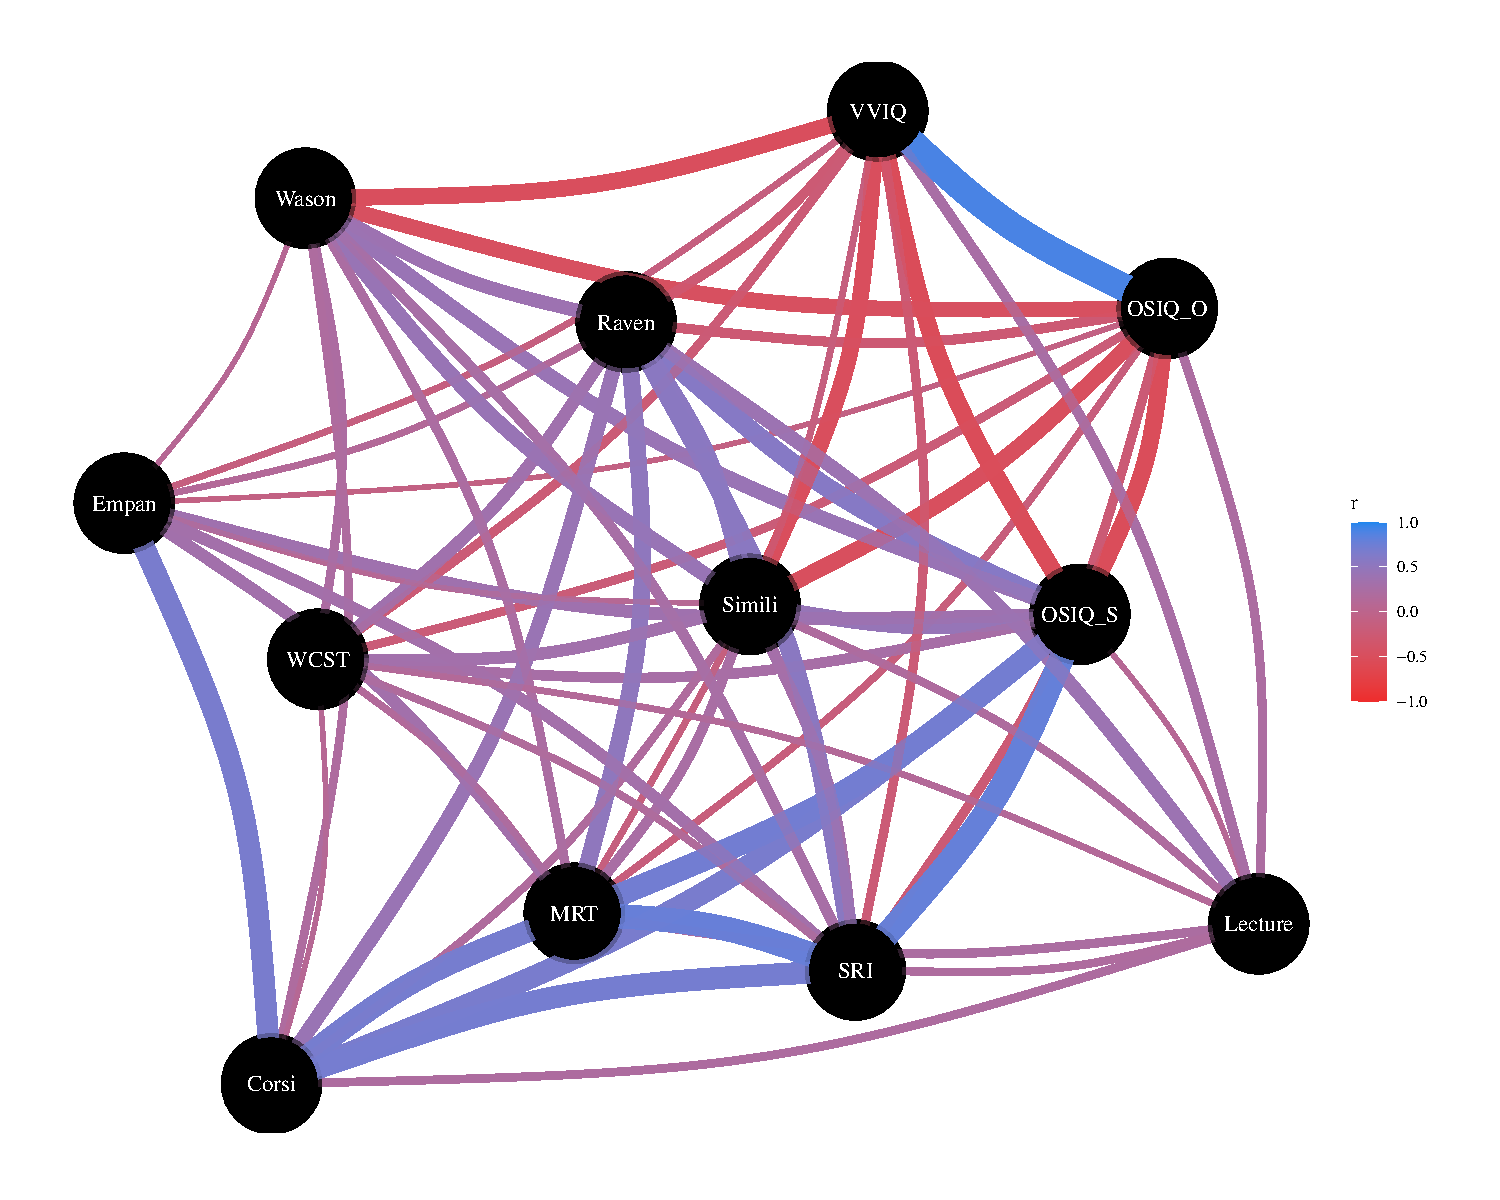
\includegraphics[width=\textwidth,height=0.5\textheight]{aphantasia_quarto_files/figure-pdf/ggm-1.pdf}

\caption{Représentation des corrélations entre les variables mesurées. Les liens bleus dénotent une corrélation positive, et les rouges une corrélation négative. Cette figure illustre les choix de pondération réalisés à l'étape de simulation : on peut notamment voir des corrélations très prononcées entre le VVIQ et l'OSIQ-objet (r = 0.77*) qui évaluent tous deux l'imagerie objet, le Digit Span et les blocs de Corsi (r = 0.68*) qui évaluent entre autres la mémoire de travail, ou encore entre l'OSIQ-spatial et le SRI, qui respectivement l'auto-évaluation et la tâche les plus spécifiques de l'imagerie spatiale.}
\label{ggm}
\end{figure}

\hypertarget{analyse-de-facteurs}{%
\subsubsection{Analyse de facteurs}\label{analyse-de-facteurs}}

\emph{check\_factorstructure} de \emph{easystats} Is the data suitable
for Factor Analysis? - KMO: The Kaiser, Meyer, Olkin (KMO) measure of
sampling adequacy suggests that data seems appropriate for factor
analysis (KMO = 0.82). - Sphericity: Bartlett's test of sphericity
suggests that there is sufficient significant correlation in the data
for factor analysis (Chisq(66) = 3194.04, p \textless{} .001).

\hypertarget{analyses-des-groupes-par-partition-non-supervisuxe9e}{%
\subsubsection{Analyses des groupes par partition
non-supervisée}\label{analyses-des-groupes-par-partition-non-supervisuxe9e}}

\begin{figure}[H]

\caption{Graphique représentatant l'évalution du nombre idéal de clusters par la méthode 'Within Sum of Squares'.}
\label{cluster_number}
\end{figure}

\begin{figure}[H]

\caption{Représentation de l'analyse en composantes principales des variables mesurées.}
\label{pca_variables}
\end{figure}

\begin{figure}[H]

\caption{Représentation des clusters reconnus par la méthode des 'k-means', selon les deux composantes principales de l'ACP.}
\label{k_means}
\end{figure}

\hypertarget{analyse-des-clusters}{%
\subsubsection{Analyse des clusters}\label{analyse-des-clusters}}

\begin{figure}[H]

\caption{Diagramme représentatant les profils cognitifs associés à chaque cluster, selon quatre dimensions principales : l'imagerie visuelle-objet, l'imagerie visuo-spatiale, le raisonnement et les fonctions exécutives.}
\label{profiles_radar}
\end{figure}

\begin{figure}[H]

\caption{Représentation alternative des profils cognitifs associés aux clusters.}
\label{profiles_lollipop}
\end{figure}

\hypertarget{comparaison-des-profils-cognitifs}{%
\subsubsection{Comparaison des profils
cognitifs}\label{comparaison-des-profils-cognitifs}}

\begin{figure}[H]

\caption{Répartion des groupes par cluster.}
\label{cluster_repatition}
\end{figure}

\begin{figure}[H]

\caption{Comparaison des moyennes de score d'imagerie visuelle-objet entre les quatre groupes identifiés.}
\label{object_img_violins}
\end{figure}

\hypertarget{diffuxe9rences-de-moyenne-des-deux-groupes}{%
\subsubsection{Différences de moyenne des deux
groupes}\label{diffuxe9rences-de-moyenne-des-deux-groupes}}

Spatial Ability Results. Aphantasic participants reported slightly lower
spatial imagery ability on the spatial sub-component of the OSIQ when
compared to control group 1 (Mann-Whitney U = 24,462, p = 0.001, r =
.15, BF10 = 14.65, two-sided; see Figure 2.1 purple section), although
this effect was not significant after Bonferroni correction.
Additionally, the scores of aphantasic individuals on the Spatial Memory
component of the SAM (which includes items measuring reported spatial
navigation and naturalistic spatial memory ability) were not
significantly different from controls (SAM; Mann-Whitney U = 24,720, p =
0.1, r = .08, BF10 = .23, two-sided; see Figure 2.1 purple section).
These results demonstrate that overall, there were no consistent
differences in reported spatial abilities between aphantasic individuals
and participants in control group 1.

Lefèvre 2022

Ptet aussi faire un tableau simple pour les moyennes générales

\hypertarget{discussion}{%
\section{Discussion}\label{discussion}}

\newpage

\hypertarget{ruxe9fuxe9rences}{%
\section*{Références}\label{ruxe9fuxe9rences}}
\addcontentsline{toc}{section}{Références}

\hypertarget{refs}{}
\begin{CSLReferences}{1}{0}
\leavevmode\vadjust pre{\hypertarget{ref-R-quarto}{}}%
Allaire, J. (2022). \emph{Quarto: {R} Interface to Quarto Markdown
Publishing System} {[}Manual{]}.
\url{https://github.com/quarto-dev/quarto-r}

\leavevmode\vadjust pre{\hypertarget{ref-R-rmarkdown}{}}%
Allaire, J., Xie, Y., McPherson, J., Luraschi, J., Ushey, K., Atkins,
A., Wickham, H., Cheng, J., Chang, W., \& Iannone, R. (2023).
\emph{Rmarkdown: {Dynamic} Documents for {R}} {[}Manual{]}.
\url{https://CRAN.R-project.org/package=rmarkdown}

\leavevmode\vadjust pre{\hypertarget{ref-R-equatiomatic}{}}%
Anderson, D., Heiss, A., \& Sumners, J. (2022). \emph{Equatiomatic:
{Transform} Models into {LaTeX} Equations} {[}Manual{]}.
\url{https://CRAN.R-project.org/package=equatiomatic}

\leavevmode\vadjust pre{\hypertarget{ref-bainbridgeQuantifyingAphantasiaDrawing2021}{}}%
Bainbridge, W. A., Pounder, Z., Eardley, A. F., \& Baker, C. I. (2021).
Quantifying Aphantasia through Drawing: {Those} without Visual Imagery
Show Deficits in Object but Not Spatial Memory. \emph{Cortex},
\emph{135}, 159‑172. \url{https://doi.org/10.1016/j.cortex.2020.11.014}

\leavevmode\vadjust pre{\hypertarget{ref-bartolomeoAssessingCausalRole2020}{}}%
Bartolomeo, P., Hajhajate, D., Liu, J., \& Spagna, A. (2020). Assessing
the Causal Role of Early Visual Areas in Visual Mental Imagery.
\emph{Nature Reviews Neuroscience}, \emph{21}(9, 9), 517‑517.
\url{https://doi.org/10.1038/s41583-020-0348-5}

\leavevmode\vadjust pre{\hypertarget{ref-R-lme4}{}}%
Bates, D., Maechler, M., Bolker, B., \& Walker, S. (2022). \emph{Lme4:
{Linear} Mixed-Effects Models Using Eigen and {S4}} {[}Manual{]}.
\url{https://github.com/lme4/lme4/}

\leavevmode\vadjust pre{\hypertarget{ref-R-Matrix}{}}%
Bates, D., Maechler, M., \& Jagan, M. (2022). \emph{Matrix: {Sparse} and
Dense Matrix Classes and Methods} {[}Manual{]}.
\url{https://CRAN.R-project.org/package=Matrix}

\leavevmode\vadjust pre{\hypertarget{ref-R-effectsize}{}}%
Ben-Shachar, M. S., Makowski, D., Lüdecke, D., Patil, I., Wiernik, B.
M., \& Th'eriault, R. (2023). \emph{Effectsize: {Indices} of Effect
Size} {[}Manual{]}. \url{https://easystats.github.io/effectsize/}

\leavevmode\vadjust pre{\hypertarget{ref-R-ggradar}{}}%
Bion, R. (2023). \emph{Ggradar: {Create} Radar Charts Using Ggplot2}
{[}Manual{]}.

\leavevmode\vadjust pre{\hypertarget{ref-blajenkovaObjectSpatialImagery2006}{}}%
Blajenkova, O., Kozhevnikov, M., \& Motes, M. A. (2006a). Object and
Spatial Imagery: Distinctions between Members of Different Professions.
\emph{Cognitive Processing}, \emph{7}(1), 20‑21.
\url{https://doi.org/10.1007/s10339-006-0047-9}

\leavevmode\vadjust pre{\hypertarget{ref-blajenkovaObjectspatialImageryNew2006}{}}%
Blajenkova, O., Kozhevnikov, M., \& Motes, M. A. (2006b). Object-Spatial
Imagery: A New Self-Report Imagery Questionnaire. \emph{Applied
Cognitive Psychology}, \emph{20}(2), 239‑263.
\url{https://doi.org/10.1002/acp.1182}

\leavevmode\vadjust pre{\hypertarget{ref-blazhenkovaVisualobjectAbilityNew2010}{}}%
Blazhenkova, O., \& Kozhevnikov, M. (2010). Visual-Object Ability: {A}
New Dimension of Non-Verbal Intelligence. \emph{Cognition},
\emph{117}(3), 276‑301.
\url{https://doi.org/10.1016/j.cognition.2010.08.021}

\leavevmode\vadjust pre{\hypertarget{ref-blazhenkovaNewObjectspatialverbalCognitive2009}{}}%
Blazhenkova, O., \& Kozhevnikov, M. (2009). The New
Object-Spatial-Verbal Cognitive Style Model: {Theory} and Measurement.
\emph{Applied Cognitive Psychology}, \emph{23}(5), 638‑663.
\url{https://doi.org/10.1002/acp.1473}

\leavevmode\vadjust pre{\hypertarget{ref-blazhenkovaTwoEyesBlind2019}{}}%
Blazhenkova, O., \& Pechenkova, E. (2019). The Two Eyes of the Blind
Mind: Object vs. Spatial Aphantasia? \emph{Russian Journal of Cognitive
Science}, \emph{6}(4, 4), 51‑65. \url{http://dx.doi.org/10.47010/19.4.5}

\leavevmode\vadjust pre{\hypertarget{ref-blomkvistAphantasiaSearchTheory2022}{}}%
Blomkvist, A. (2022). Aphantasia: {In} Search of a Theory. \emph{Mind \&
Language}, \emph{n/a}(n/a). \url{https://doi.org/10.1111/mila.12432}

\leavevmode\vadjust pre{\hypertarget{ref-bocciaPennyYourThoughts2015}{}}%
Boccia, M., Piccardi, L., Palermo, L., Nemmi, F., Sulpizio, V., Galati,
G., \& Guariglia, C. (2015). A Penny for Your Thoughts! Patterns of
{fMRI} Activity Reveal the Content and the Spatial Topography of Visual
Mental Images. \emph{Human Brain Mapping}, \emph{36}(3), 945‑958.
\url{https://doi.org/10.1002/hbm.22678}

\leavevmode\vadjust pre{\hypertarget{ref-brewerScientistsAreNot2006}{}}%
Brewer, W. F., \& Schommer-Aikins, M. (2006). Scientists {Are Not
Deficient} in {Mental Imagery}: {Galton Revised}. \emph{Review of
General Psychology}, \emph{10}(2), 130‑146.
\url{https://doi.org/10.1037/1089-2680.10.2.130}

\leavevmode\vadjust pre{\hypertarget{ref-cavedon-taylorPredictiveProcessingPerception2021}{}}%
Cavedon-Taylor, D. (2021). \emph{Predictive {Processing} and
{Perception}: {What} Does {Imagining} Have to Do with It?} 15.

\leavevmode\vadjust pre{\hypertarget{ref-colemanSpatialPerceptionSkills1998}{}}%
Coleman, S. L., \& Gotch, A. J. (1998). Spatial {Perception Skills} of
{Chemistry Students}. \emph{Journal of Chemical Education},
\emph{75}(2), 206. \url{https://doi.org/10.1021/ed075p206}

\leavevmode\vadjust pre{\hypertarget{ref-crowderDifferencesSpatialVisualization2018}{}}%
Crowder, A. (2018). \emph{Differences in {Spatial Visualization Ability}
and {Vividness} of {Spatial Imagery Between People With} and {Without
Aphantasia}}.

\leavevmode\vadjust pre{\hypertarget{ref-igraph2006}{}}%
Csardi, G., \& Nepusz, T. (2006). The Igraph Software Package for
Complex Network Research. \emph{InterJournal}, \emph{Complex Systems},
1695. \url{https://igraph.org}

\leavevmode\vadjust pre{\hypertarget{ref-danceLessSensoryOverwhelm2022}{}}%
Dance, C. (2022, janvier 26). \emph{Less {Sensory Overwhelm In
Aphantasia}: {A Potential Advantage}?}
\url{https://aphantasia.com/sensory-overwhelm/}

\leavevmode\vadjust pre{\hypertarget{ref-dancePrevalenceAphantasiaImagery2022}{}}%
Dance, C. J., Ipser, A., \& Simner, J. (2022). The Prevalence of
Aphantasia (Imagery Weakness) in the General Population.
\emph{Consciousness and Cognition}, \emph{97}, 103243.
\url{https://doi.org/10.1016/j.concog.2021.103243}

\leavevmode\vadjust pre{\hypertarget{ref-danceWhatLinkMental2021}{}}%
Dance, C. J., Ward, J., \& Simner, J. (2021). What Is the {Link Between
Mental Imagery} and {Sensory Sensitivity}? {Insights} from {Aphantasia}.
\emph{Perception}, \emph{50}(9), 757‑782.
\url{https://doi.org/10.1177/03010066211042186}

\leavevmode\vadjust pre{\hypertarget{ref-dawesInnerVisionsMind2022}{}}%
Dawes, A. (2022). \emph{Inner Visions of the Mind's Eye: {The} Role of
Visual Imagery in Remembering the Past and Imagining the Future}
{[}{UNSW Sydney}{]}. \url{https://doi.org/10.26190/UNSWORKS/24158}

\leavevmode\vadjust pre{\hypertarget{ref-dawesCognitiveProfileMultisensory2020}{}}%
Dawes, A. J., Keogh, R., Andrillon, T., \& Pearson, J. (2020). A
Cognitive Profile of Multi-Sensory Imagery, Memory and Dreaming in
Aphantasia. \emph{Scientific Reports}, \emph{10}(1, 1), 10022.
\url{https://doi.org/10.1038/s41598-020-65705-7}

\leavevmode\vadjust pre{\hypertarget{ref-dellasalaPatternSpanTool1999}{}}%
Della Sala, S., Gray, C., Baddeley, A., Allamano, N., \& Wilson, L.
(1999). Pattern Span: A Tool for Unwelding Visuo--Spatial Memory.
\emph{Neuropsychologia}, \emph{37}(10), 1189‑1199.
\url{https://doi.org/10.1016/S0028-3932(98)00159-6}

\leavevmode\vadjust pre{\hypertarget{ref-R-pandoc}{}}%
Dervieux, C. (2022). \emph{Pandoc: {Manage} and Run Universal Converter
Pandoc from {R}} {[}Manual{]}.
\url{https://CRAN.R-project.org/package=pandoc}

\leavevmode\vadjust pre{\hypertarget{ref-farahCaseStudyMental1988}{}}%
Farah, M. J., Levine, D. N., \& Calvanio, R. (1988). A Case Study of
Mental Imagery Deficit. \emph{Brain and Cognition}, \emph{8}(2),
147‑164. \url{https://doi.org/10.1016/0278-2626(88)90046-2}

\leavevmode\vadjust pre{\hypertarget{ref-fawConflictingIntuitionsMay2009}{}}%
Faw, B. (2009). \emph{Conflicting {Intuitions May Be Based On Differing
Abilities}}. 25.

\leavevmode\vadjust pre{\hypertarget{ref-fox-muratonWorldImaginationConsequences2021}{}}%
Fox-Muraton, M. (2021). A World without Imagination? {Consequences} of
Aphantasia for an Existential Account of Self. \emph{History of European
Ideas}, \emph{47}(3), 414‑428.
\url{https://doi.org/10.1080/01916599.2020.1799553}

\leavevmode\vadjust pre{\hypertarget{ref-galtonSTATISTICSMENTALIMAGERY1880}{}}%
Galton, F. (1880). I.---{STATISTICS OF MENTAL IMAGERY}. \emph{Mind},
\emph{os-V}(19), 301‑318. \url{https://doi.org/10.1093/mind/os-V.19.301}

\leavevmode\vadjust pre{\hypertarget{ref-greenbergRoleVisualImagery2014}{}}%
Greenberg, D. L., \& Knowlton, B. J. (2014). The Role of Visual Imagery
in Autobiographical Memory. \emph{Memory \& Cognition}, \emph{42}(6),
922‑934. \url{https://doi.org/10.3758/s13421-014-0402-5}

\leavevmode\vadjust pre{\hypertarget{ref-hegartyIndividualDifferencesSpatial2005}{}}%
Hegarty, M., \& Waller, D. A. (2005). Individual {Differences} in
{Spatial Abilities}. In \emph{The {Cambridge Handbook} of {Visuospatial
Thinking}} (p. 121‑169). {Cambridge University Press}.
\url{https://doi.org/10.1017/CBO9780511610448.005}

\leavevmode\vadjust pre{\hypertarget{ref-R-purrr}{}}%
Henry, L., \& Wickham, H. (2022). \emph{Purrr: {Functional} Programming
Tools} {[}Manual{]}. \url{https://CRAN.R-project.org/package=purrr}

\leavevmode\vadjust pre{\hypertarget{ref-R-ggpubr}{}}%
Kassambara, A. (2022a). \emph{Ggpubr: Ggplot2 Based Publication Ready
Plots} {[}Manual{]}. \url{https://rpkgs.datanovia.com/ggpubr/}

\leavevmode\vadjust pre{\hypertarget{ref-R-rstatix}{}}%
Kassambara, A. (2022b). \emph{Rstatix: {Pipe-friendly} Framework for
Basic Statistical Tests} {[}Manual{]}.
\url{https://rpkgs.datanovia.com/rstatix/}

\leavevmode\vadjust pre{\hypertarget{ref-R-factoextra}{}}%
Kassambara, A., \& Mundt, F. (2020). \emph{Factoextra: {Extract} and
Visualize the Results of Multivariate Data Analyses} {[}Manual{]}.
\url{http://www.sthda.com/english/rpkgs/factoextra}

\leavevmode\vadjust pre{\hypertarget{ref-keehnerSpatialAbilityExperience2004}{}}%
Keehner, M. M., Tendick, F., Meng, M. V., Anwar, H. P., Hegarty, M.,
Stoller, M. L., \& Duh, Q.-Y. (2004). Spatial Ability, Experience, and
Skill in Laparoscopic Surgery. \emph{The American Journal of Surgery},
\emph{188}(1), 71‑75.
\url{https://doi.org/10.1016/j.amjsurg.2003.12.059}

\leavevmode\vadjust pre{\hypertarget{ref-kendleAphantasiaExperiencesPerceptions2017}{}}%
Kendle, A. (2017). \emph{Aphantasia: {Experiences}, Perceptions, and
Insights}. {Dark River}.

\leavevmode\vadjust pre{\hypertarget{ref-keoghBlindMindNo2018}{}}%
Keogh, R., \& Pearson, J. (2018). The Blind Mind: {No} Sensory Visual
Imagery in Aphantasia. \emph{Cortex}, \emph{105}, 53‑60.
\url{https://doi.org/10.1016/j.cortex.2017.10.012}

\leavevmode\vadjust pre{\hypertarget{ref-keoghAttentionDrivenPhantom2020}{}}%
Keogh, R., \& Pearson, J. (2020). Attention Driven Phantom Vision:
Measuring the Sensory Strength of Attentional Templates and Their
Relation to Visual Mental Imagery and Aphantasia. \emph{Philosophical
Transactions of the Royal Society B: Biological Sciences},
\emph{376}(1817), 20190688. \url{https://doi.org/10.1098/rstb.2019.0688}

\leavevmode\vadjust pre{\hypertarget{ref-keoghVisualWorkingMemory2021}{}}%
Keogh, R., Wicken, M., \& Pearson, J. (2021). Visual Working Memory in
Aphantasia: {Retained} Accuracy and Capacity with a Different Strategy.
\emph{Cortex}, \emph{143}, 237‑253.
\url{https://doi.org/10.1016/j.cortex.2021.07.012}

\leavevmode\vadjust pre{\hypertarget{ref-knightMemoryImageryNo2022}{}}%
Knight, K. F., Milton, F. N., Milton, F. N., Zeman, A., \& Zeman, A.
(2022). \emph{Memory without {Imagery}: {No Evidence} of {Visual Working
Memory Impairment} in {People} with {Aphantasia}}. 8.

\leavevmode\vadjust pre{\hypertarget{ref-kosslynCognitiveNeuroscienceMental1995}{}}%
Kosslyn, S. M., Behrmann, M., \& Jeannerod, M. (1995). The Cognitive
Neuroscience of Mental Imagery. \emph{Neuropsychologia}, \emph{33}(11),
1335‑1344. \url{https://doi.org/10.1016/0028-3932(95)00067-D}

\leavevmode\vadjust pre{\hypertarget{ref-kotheTrackdownCollaborativeWriting2021}{}}%
Kothe, E., Callegher, C. Z., Gambarota, F., Linkersdörfer, J., \& Ling,
M. (2021). \emph{Trackdown: {Collaborative Writing} and {Editing} of {R
Markdown} (or {Sweave}) {Documents} in {Google Drive}}. {Zenodo}.
\url{https://doi.org/10.5281/zenodo.5167320}

\leavevmode\vadjust pre{\hypertarget{ref-kozhevnikovTradeoffObjectSpatial2010}{}}%
Kozhevnikov, M., Blazhenkova, O., \& Becker, M. (2010). Trade-off in
Object versus Spatial Visualization Abilities: {Restriction} in the
Development of Visual-Processing Resources. \emph{Psychonomic Bulletin
\& Review}, \emph{17}(1), 29‑35.
\url{https://doi.org/10.3758/PBR.17.1.29}

\leavevmode\vadjust pre{\hypertarget{ref-kozhevnikovRevisingVisualizerVerbalizerDimension2002}{}}%
Kozhevnikov, M., Hegarty, M., \& Mayer, R. E. (2002). Revising the
{Visualizer-Verbalizer Dimension}: {Evidence} for {Two Types} of
{Visualizers}. \emph{Cognition and Instruction}, \emph{20}(1), 47‑77.
\url{https://www.jstor.org/stable/3233862}

\leavevmode\vadjust pre{\hypertarget{ref-kozhevnikovSpatialObjectVisualizers2005}{}}%
Kozhevnikov, M., Kosslyn, S., \& Shephard, J. (2005). Spatial versus
Object Visualizers: {A} New Characterization of Visual Cognitive Style.
\emph{Memory \& Cognition}, \emph{33}(4), 710‑726.
\url{https://doi.org/10.3758/BF03195337}

\leavevmode\vadjust pre{\hypertarget{ref-kozhevnikovCreativityVisualizationAbilities2013}{}}%
Kozhevnikov, M., Kozhevnikov, M., Yu, C. J., \& Blazhenkova, O. (2013).
Creativity, Visualization Abilities, and Visual Cognitive Style.
\emph{British Journal of Educational Psychology}, \emph{83}(2), 196‑209.
\url{https://doi.org/10.1111/bjep.12013}

\leavevmode\vadjust pre{\hypertarget{ref-kozhevnikovSpatialVisualizationPhysics2007}{}}%
Kozhevnikov, M., Motes, M. A., \& Hegarty, M. (2007). Spatial
{Visualization} in {Physics Problem Solving}. \emph{Cognitive Science},
\emph{31}(4), 549‑579. \url{https://doi.org/10.1080/15326900701399897}

\leavevmode\vadjust pre{\hypertarget{ref-R-corrr}{}}%
Kuhn, M., Jackson, S., \& Cimentada, J. (2022). \emph{Corrr:
{Correlations} in {R}} {[}Manual{]}.
\url{https://CRAN.R-project.org/package=corrr}

\leavevmode\vadjust pre{\hypertarget{ref-R-lmerTest}{}}%
Kuznetsova, A., Bruun Brockhoff, P., \& Haubo Bojesen Christensen, R.
(2020). \emph{{lmerTest}: {Tests} in Linear Mixed Effects Models}
{[}Manual{]}. \url{https://github.com/runehaubo/lmerTestR}

\leavevmode\vadjust pre{\hypertarget{ref-lachlanPupillaryLightResponse2022}{}}%
Lachlan, K., Keogh, R., Andrillion, T., \& Pearson, J. (2022, mars 31).
\emph{The Pupillary Light Response as a Physiological Index of
Aphantasia, Sensory and Phenomenological Imagery Strength \textbar{}
{eLife}}. \url{https://elifesciences.org/articles/72484}

\leavevmode\vadjust pre{\hypertarget{ref-langeJustAnotherTool2015}{}}%
Lange, K., Kühn, S., \& Filevich, E. (2015). {Just Another Tool} for
{Online Studies}'' ({JATOS}): {An Easy Solution} for {Setup} and
{Management} of {Web Servers Supporting Online Studies}. \emph{PLOS
ONE}, \emph{10}(6), e0130834.
\url{https://doi.org/10.1371/journal.pone.0130834}

\leavevmode\vadjust pre{\hypertarget{ref-R-ez}{}}%
Lawrence, M. A. (2016). \emph{Ez: {Easy} Analysis and Visualization of
Factorial Experiments} {[}Manual{]}.
\url{http://github.com/mike-lawrence/ez}

\leavevmode\vadjust pre{\hypertarget{ref-R-easystats}{}}%
Lüdecke, D., Makowski, D., Ben-Shachar, M. S., Patil, I., \& Wiernik, B.
M. (2022). \emph{Easystats: {Framework} for Easy Statistical Modeling,
Visualization, and Reporting} {[}Manual{]}.
\url{https://easystats.github.io/easystats/}

\leavevmode\vadjust pre{\hypertarget{ref-R-insight}{}}%
Lüdecke, D., Makowski, D., Patil, I., Waggoner, P., Ben-Shachar, M. S.,
Wiernik, B. M., \& Arel-Bundock, V. (2023). \emph{Insight: {Easy} Access
to Model Information for Various Model Objects} {[}Manual{]}.
\url{https://easystats.github.io/insight/}

\leavevmode\vadjust pre{\hypertarget{ref-R-cluster}{}}%
Maechler, M., Rousseeuw, P., Struyf, A., \& Hubert, M. (2022).
\emph{Cluster: "{Finding Groups} in {Data}": {Cluster} Analysis Extended
Rousseeuw et Al.} {[}Manual{]}.
\url{https://svn.r-project.org/R-packages/trunk/cluster/}

\leavevmode\vadjust pre{\hypertarget{ref-R-modelbased}{}}%
Makowski, D., Lüdecke, D., Ben-Shachar, M. S., \& Patil, I. (2023).
\emph{Modelbased: {Estimation} of Model-Based Predictions, Contrasts and
Means} {[}Manual{]}. \url{https://easystats.github.io/modelbased/}

\leavevmode\vadjust pre{\hypertarget{ref-R-correlation}{}}%
Makowski, D., Wiernik, B. M., Patil, I., Lüdecke, D., \& Ben-Shachar, M.
S. (2022). \emph{Correlation: {Methods} for Correlation Analysis}
{[}Manual{]}. \url{https://easystats.github.io/correlation/}

\leavevmode\vadjust pre{\hypertarget{ref-marksVividnessVisualImagery1973}{}}%
Marks, D. F. (1973). Vividness of Visual Imagery {Questionnaire}.
\emph{Journal of Mental Imagery}.

\leavevmode\vadjust pre{\hypertarget{ref-mathotOpenSesameOpensourceGraphical2012}{}}%
Mathôt, S., Schreij, D., \& Theeuwes, J. (2012). {OpenSesame}: {An}
Open-Source, Graphical Experiment Builder for the Social Sciences.
\emph{Behavior Research Methods}, \emph{44}(2), 314‑324.
\url{https://doi.org/10.3758/s13428-011-0168-7}

\leavevmode\vadjust pre{\hypertarget{ref-miltonBehavioralNeuralSignatures2021}{}}%
Milton, F., Fulford, J., Dance, C., Gaddum, J., Heuerman-Williamson, B.,
Jones, K., Knight, K. F., MacKisack, M., Winlove, C., \& Zeman, A.
(2021). Behavioral and {Neural Signatures} of {Visual Imagery Vividness
Extremes}: {Aphantasia} versus {Hyperphantasia}. \emph{Cerebral Cortex
Communications}, \emph{2}(2), tgab035.
\url{https://doi.org/10.1093/texcom/tgab035}

\leavevmode\vadjust pre{\hypertarget{ref-mishkinContributionStriateInputs1982}{}}%
Mishkin, M., \& Ungerleider, L. G. (1982). Contribution of Striate
Inputs to the Visuospatial Functions of Parieto-Preoccipital Cortex in
Monkeys. \emph{Behavioural Brain Research}, \emph{6}(1), 57‑77.
\url{https://doi.org/10.1016/0166-4328(82)90081-X}

\leavevmode\vadjust pre{\hypertarget{ref-monzelAphantasiaDysikonesiaAnauralia2022}{}}%
Monzel, M., Mitchell, D., Macpherson, F., Pearson, J., \& Zeman, A.
(2022). Aphantasia, Dysikonesia, Anauralia: Call for a Single Term for
the Lack of Mental Imagery--{Commentary} on {Dance} et~al. (2021) and
{Hinwar} and {Lambert} (2021). \emph{Cortex}, \emph{150}, 149‑152.
\url{https://doi.org/10.1016/j.cortex.2022.02.002}

\leavevmode\vadjust pre{\hypertarget{ref-mortonImageTransformationDissociated1995}{}}%
Morton, N., \& Morris, R. G. (1995). Image Transformation Dissociated
from Visuospatial Working Memory. \emph{Cognitive Neuropsychology},
\emph{12}(7), 767‑791. \url{https://doi.org/10.1080/02643299508251401}

\leavevmode\vadjust pre{\hypertarget{ref-orionRelationshipEarthScienceEducation1997}{}}%
Orion, N., Ben-Chaim, D., \& Kali, Y. (1997). Relationship {Between
Earth-Science Education} and {Spatial Visualization}. \emph{Journal of
Geoscience Education}, \emph{45}(2), 129‑132.
\url{https://doi.org/10.5408/1089-9995-45.2.129}

\leavevmode\vadjust pre{\hypertarget{ref-palermoCongenitalLackExtraordinary2022}{}}%
Palermo, L., Boccia, M., Piccardi, L., \& Nori, R. (2022). Congenital
Lack and Extraordinary Ability in Object and Spatial Imagery: {An}
Investigation on Sub-Types of Aphantasia and Hyperphantasia.
\emph{Consciousness and Cognition}, \emph{103}, 103360.
\url{https://doi.org/10.1016/j.concog.2022.103360}

\leavevmode\vadjust pre{\hypertarget{ref-datawizard2022}{}}%
Patil, I., Makowski, D., Ben-Shachar, M. S., Wiernik, B. M., Bacher, E.,
\& Lüdecke, D. (2022). {datawizard}: {An R} Package for Easy Data
Preparation and Statistical Transformations. \emph{Journal of Open
Source Software}, \emph{7}(78), 4684.
\url{https://doi.org/10.21105/joss.04684}

\leavevmode\vadjust pre{\hypertarget{ref-pearsonHumanImaginationCognitive2019}{}}%
Pearson, J. (2019). The Human Imagination: The Cognitive Neuroscience of
Visual Mental Imagery. \emph{Nature Reviews Neuroscience}, \emph{20}(10,
10), 624‑634. \url{https://doi.org/10.1038/s41583-019-0202-9}

\leavevmode\vadjust pre{\hypertarget{ref-R-ggraph}{}}%
Pedersen, T. L. (2022). \emph{Ggraph: {An} Implementation of Grammar of
Graphics for Graphs and Networks} {[}Manual{]}.
\url{https://CRAN.R-project.org/package=ggraph}

\leavevmode\vadjust pre{\hypertarget{ref-positteamRStudioIntegratedDevelopment2022}{}}%
Posit team. (2022). \emph{{RStudio}: {Integrated} Development
Environment for {R}} {[}Manual{]}. {Posit Software, PBC}.
\url{http://www.posit.co/}

\leavevmode\vadjust pre{\hypertarget{ref-pounderOnlyMinimalDifferences2022}{}}%
Pounder, Z., Jacob, J., Evans, S., Loveday, C., Eardley, A. F., \&
Silvanto, J. (2022). Only Minimal Differences between Individuals with
Congenital Aphantasia and Those with Typical Imagery on
Neuropsychological Tasks That Involve Imagery. \emph{Cortex},
\emph{148}, 180‑192. \url{https://doi.org/10.1016/j.cortex.2021.12.010}

\leavevmode\vadjust pre{\hypertarget{ref-pylyshynMentalImagerySearch2002}{}}%
Pylyshyn, Z. W. (2002). Mental Imagery: {In} Search of a Theory.
\emph{Behavioral and Brain Sciences}, \emph{25}(2), 157‑182.
\url{https://doi.org/10.1017/S0140525X02000043}

\leavevmode\vadjust pre{\hypertarget{ref-R-librarian}{}}%
Quintans, D. (2021). \emph{Librarian: {Install}, Update, Load Packages
from {CRAN}, {GitHub}, and Bioconductor in One Step} {[}Manual{]}.
\url{https://github.com/DesiQuintans/librarian}

\leavevmode\vadjust pre{\hypertarget{ref-R-base}{}}%
R Core Team. (2022). \emph{R: {A} Language and Environment for
Statistical Computing} {[}Manual{]}. {R Foundation for Statistical
Computing}. \url{https://www.R-project.org/}

\leavevmode\vadjust pre{\hypertarget{ref-reisbergIntuitionsIntrospectionsImagery2002}{}}%
Reisberg, D., Pearson, D. G., \& Kosslyn, S. M. (2002). Intuitions and
Introspections about Imagery: The Role of Imagery Experience in Shaping
an Investigator's Theoretical Views. \emph{Applied Cognitive
Psychology}, \emph{17}(2), 147‑160.
\url{https://doi.org/10.1002/acp.858}

\leavevmode\vadjust pre{\hypertarget{ref-R-MASS}{}}%
Ripley, B. (2022). \emph{{MASS}: {Support} Functions and Datasets for
Venables and Ripley's {MASS}} {[}Manual{]}.
\url{http://www.stats.ox.ac.uk/pub/MASS4/}

\leavevmode\vadjust pre{\hypertarget{ref-salwayVisuospatialWorkingMemory1995}{}}%
Salway, A. F. S., \& Logie, R. H. (1995). Visuospatial Working Memory,
Movement Control and Executive Demands. \emph{British Journal of
Psychology}, \emph{86}(2), 253‑269.
\url{https://doi.org/10.1111/j.2044-8295.1995.tb02560.x}

\leavevmode\vadjust pre{\hypertarget{ref-R-GGally}{}}%
Schloerke, B., Cook, D., Larmarange, J., Briatte, F., Marbach, M.,
Thoen, E., Elberg, A., \& Crowley, J. (2021). \emph{{GGally}:
{Extension} to Ggplot2} {[}Manual{]}.
\url{https://CRAN.R-project.org/package=GGally}

\leavevmode\vadjust pre{\hypertarget{ref-spagnaChapterVisualMental2022}{}}%
Spagna, A. (2022). Chapter 8 - {Visual} Mental Imagery: {Inside} the
Mind's Eyes. In G. Miceli, P. Bartolomeo, \& V. Navarro (Éds.),
\emph{Handbook of {Clinical Neurology}} (Vol. 187, p. 145‑160).
{Elsevier}. \url{https://doi.org/10.1016/B978-0-12-823493-8.00010-9}

\leavevmode\vadjust pre{\hypertarget{ref-takahashiDiversityAphantasiaRevealed2022}{}}%
Takahashi, J., Saito, G., Omura, K., Yasunaga, D., Sugimura, S.,
Sakamoto, S., Horikawa, T., \& Gyoba, J. (2022). \emph{Diversity of
Aphantasia Revealed by Multiple Assessments of the Capability for
Multi-Sensory Imagery}. {PsyArXiv}.
\url{https://doi.org/10.31234/osf.io/pucsm}

\leavevmode\vadjust pre{\hypertarget{ref-waiSpatialAbilitySTEM2009}{}}%
Wai, J., Lubinski, D., \& Benbow, C. P. (2009). Spatial Ability for
{STEM} Domains: {Aligning} over 50 Years of Cumulative Psychological
Knowledge Solidifies Its Importance. \emph{Journal of Educational
Psychology}, \emph{101}, 817‑835. \url{https://doi.org/10.1037/a0016127}

\leavevmode\vadjust pre{\hypertarget{ref-watkinsPhantasiaSeverelyDeficient2018}{}}%
Watkins, N. W. (2018). ({A})Phantasia and Severely Deficient
Autobiographical Memory: {Scientific} and Personal Perspectives.
\emph{Cortex}, \emph{105}, 41‑52.
\url{https://doi.org/10.1016/j.cortex.2017.10.010}

\leavevmode\vadjust pre{\hypertarget{ref-R-forcats}{}}%
Wickham, H. (2022a). \emph{Forcats: {Tools} for Working with Categorical
Variables (Factors)} {[}Manual{]}.
\url{https://CRAN.R-project.org/package=forcats}

\leavevmode\vadjust pre{\hypertarget{ref-R-tidyverse}{}}%
Wickham, H. (2022b). \emph{Tidyverse: {Easily} Install and Load the
Tidyverse} {[}Manual{]}.
\url{https://CRAN.R-project.org/package=tidyverse}

\leavevmode\vadjust pre{\hypertarget{ref-tidyverse2019}{}}%
Wickham, H., Averick, M., Bryan, J., Chang, W., McGowan, L. D.,
François, R., Grolemund, G., Hayes, A., Henry, L., Hester, J., Kuhn, M.,
Pedersen, T. L., Miller, E., Bache, S. M., Müller, K., Ooms, J.,
Robinson, D., Seidel, D. P., Spinu, V., \ldots{} Yutani, H. (2019).
Welcome to the {tidyverse}. \emph{Journal of Open Source Software},
\emph{4}(43), 1686. \url{https://doi.org/10.21105/joss.01686}

\leavevmode\vadjust pre{\hypertarget{ref-R-dplyr}{}}%
Wickham, H., François, R., Henry, L., \& Müller, K. (2022). \emph{Dplyr:
{A} Grammar of Data Manipulation} {[}Manual{]}.
\url{https://CRAN.R-project.org/package=dplyr}

\leavevmode\vadjust pre{\hypertarget{ref-R-tidyr}{}}%
Wickham, H., \& Girlich, M. (2022). \emph{Tidyr: {Tidy} Messy Data}
{[}Manual{]}. \url{https://CRAN.R-project.org/package=tidyr}

\leavevmode\vadjust pre{\hypertarget{ref-knitr2014}{}}%
Xie, Y. (2014). Knitr: {A} Comprehensive Tool for Reproducible Research
in {R}. In V. Stodden, F. Leisch, \& R. D. Peng (Éds.),
\emph{Implementing Reproducible Computational Research}. {Chapman and
Hall/CRC}.

\leavevmode\vadjust pre{\hypertarget{ref-knitr2015}{}}%
Xie, Y. (2015). \emph{Dynamic Documents with {R} and Knitr}. {Chapman
and Hall/CRC}.

\leavevmode\vadjust pre{\hypertarget{ref-R-knitr}{}}%
Xie, Y. (2023). \emph{Knitr: {A} General-Purpose Package for Dynamic
Report Generation in {R}} {[}Manual{]}. \url{https://yihui.org/knitr/}

\leavevmode\vadjust pre{\hypertarget{ref-zagoCharcotBernardCase2011}{}}%
Zago, S., Allegri, N., Cristoffanini, M., Ferrucci, R., Porta, M., \&
Priori, A. (2011). Is the {Charcot} and {Bernard} Case (1883) of Loss of
Visual Imagery Really Based on Neurological Impairment? \emph{Cognitive
Neuropsychiatry}, \emph{16}(6), 481‑504.
\url{https://doi.org/10.1080/13546805.2011.556024}

\leavevmode\vadjust pre{\hypertarget{ref-zemanLossImageryPhenomenology2010}{}}%
Zeman, A. Z. J., Della Sala, S., Torrens, L. A., Gountouna, V.-E.,
McGonigle, D. J., \& Logie, R. H. (2010). Loss of Imagery Phenomenology
with Intact Visuo-Spatial Task Performance: {A} Case of {«~Blind
Imagination~»}. \emph{Neuropsychologia}, \emph{48}(1), 145‑155.
\url{https://doi.org/10.1016/j.neuropsychologia.2009.08.024}

\leavevmode\vadjust pre{\hypertarget{ref-zemanLivesImageryCongenital2015}{}}%
Zeman, A., Dewar, M., \& Della Sala, S. (2015). Lives without Imagery --
{Congenital} Aphantasia. \emph{Cortex}, \emph{73}, 378‑380.
\url{https://doi.org/10.1016/j.cortex.2015.05.019}

\leavevmode\vadjust pre{\hypertarget{ref-zemanPhantasiaPsychologicalSignificance2020}{}}%
Zeman, A., Milton, F., Della Sala, S., Dewar, M., Frayling, T., Gaddum,
J., Hattersley, A., Heuerman-Williamson, B., Jones, K., MacKisack, M.,
\& Winlove, C. (2020). Phantasia--{The} Psychological Significance of
Lifelong Visual Imagery Vividness Extremes. \emph{Cortex}, \emph{130},
426‑440. \url{https://doi.org/10.1016/j.cortex.2020.04.003}

\leavevmode\vadjust pre{\hypertarget{ref-zimmerBrainLookDeep2010}{}}%
Zimmer, C. (2010, mars 23). \emph{The {Brain}: {Look Deep Into} the
{Mind}'s {Eye}}. {Discover Magazine}.
\url{https://www.discovermagazine.com/mind/the-brain-look-deep-into-the-minds-eye}

\end{CSLReferences}

\newpage

\hypertarget{annexes}{%
\section*{Annexes}\label{annexes}}
\addcontentsline{toc}{section}{Annexes}

Ce manuscrit a été rédigé avec \href{https://rmarkdown.rstudio.com}{R
Markdown} (\protect\hyperlink{ref-R-rmarkdown}{Allaire et al., 2023}),
\href{https://pandoc.org/}{Pandoc}
(\protect\hyperlink{ref-R-pandoc}{Dervieux, 2022}),
\href{https://quarto.org/}{Quarto}
(\protect\hyperlink{ref-R-quarto}{Allaire, 2022}) et en \LaTeX, médiés
par le package \emph{knitr} (\protect\hyperlink{ref-knitr2014}{Xie,
2014}, \protect\hyperlink{ref-knitr2015}{2015},
\protect\hyperlink{ref-R-knitr}{2023}), dans l'Environnement de
Développement Intégré (IDE) \href{https://posit.co/}{RStudio}
(\protect\hyperlink{ref-positteamRStudioIntegratedDevelopment2022}{Posit
team, 2022}). Il a été partagé entre collaborateurs à l'aide du package
\emph{trackdown}
(\protect\hyperlink{ref-kotheTrackdownCollaborativeWriting2021}{Kothe et
al., 2021}) et de \href{https://github.com/}{\emph{GitHub}}. Le code
complet de ce manuscrit, de la simulation, des figures, tables et
analyses est accessible dans
\href{https://github.com/m-delem/aphantasia_project.git}{\emph{le
dossier de ce projet sur GitHub}}.

La préparation du code, la simulation, les figures, tables et analyses
ont nécessité les packages \emph{cluster}
(\protect\hyperlink{ref-R-cluster}{Maechler et al., 2022}),
\emph{correlation} (\protect\hyperlink{ref-R-correlation}{Makowski et
al., 2022}), \emph{corrr} (\protect\hyperlink{ref-R-corrr}{Kuhn et al.,
2022}), \emph{datawizard} (\protect\hyperlink{ref-datawizard2022}{Patil
et al., 2022}), \emph{dplyr} (\protect\hyperlink{ref-R-dplyr}{Wickham et
al., 2022}), \emph{easystats}
(\protect\hyperlink{ref-R-easystats}{Lüdecke et al., 2022}),
\emph{effectsize} (\protect\hyperlink{ref-R-effectsize}{Ben-Shachar et
al., 2023}), \emph{equatiomatic}
(\protect\hyperlink{ref-R-equatiomatic}{Anderson et al., 2022}),
\emph{ez} (\protect\hyperlink{ref-R-ez}{Lawrence, 2016}),
\emph{factoextra} (\protect\hyperlink{ref-R-factoextra}{Kassambara \&
Mundt, 2020}), \emph{forcats}
(\protect\hyperlink{ref-R-forcats}{Wickham, 2022a}), \emph{GGally}
(\protect\hyperlink{ref-R-GGally}{Schloerke et al., 2021}),
\emph{ggpubr} (\protect\hyperlink{ref-R-ggpubr}{Kassambara, 2022a}),
\emph{ggradar} (\protect\hyperlink{ref-R-ggradar}{Bion, 2023}),
\emph{ggraph} (\protect\hyperlink{ref-R-ggraph}{Pedersen, 2022}),
\emph{igraph} (\protect\hyperlink{ref-igraph2006}{Csardi \& Nepusz,
2006}), \emph{insight} (\protect\hyperlink{ref-R-insight}{Lüdecke et
al., 2023}), \emph{librarian}
(\protect\hyperlink{ref-R-librarian}{Quintans, 2021}), \emph{lme4}
(\protect\hyperlink{ref-R-lme4}{Bates, Maechler, Bolker, et al., 2022}),
\emph{lmerTest} (\protect\hyperlink{ref-R-lmerTest}{Kuznetsova et al.,
2020}), \emph{MASS} (\protect\hyperlink{ref-R-MASS}{Ripley, 2022}),
\emph{Matrix} (\protect\hyperlink{ref-R-Matrix}{Bates, Maechler, \&
Jagan, 2022}), \emph{modelbased}
(\protect\hyperlink{ref-R-modelbased}{Makowski et al., 2023}),
\emph{purrr} (\protect\hyperlink{ref-R-purrr}{Henry \& Wickham, 2022}),
\emph{rstatix} (\protect\hyperlink{ref-R-rstatix}{Kassambara, 2022b}),
\emph{tidyr} (\protect\hyperlink{ref-R-tidyr}{Wickham \& Girlich,
2022}), et \emph{tidyverse}
(\protect\hyperlink{ref-tidyverse2019}{Wickham et al., 2019};
\protect\hyperlink{ref-R-tidyverse}{Wickham, 2022b}).



\end{document}
